\documentclass[11pt]{article}

% this is the template for an issue of the Data Engineering Bulletin
\usepackage{deauthor,times,graphicx}


% all packages used by any paper must be listed here

% \usepackage{latexsym}

% For proper rendering and hyphenation of words containing Latin characters (including in bib files)
% \usepackage[T1]{fontenc}
% For Vietnamese characters
% \usepackage[T5]{fontenc}
% See https://www.latex-project.org/help/documentation/encguide.pdf for other character sets

% This assumes your files are encoded as UTF8
%\usepackage[utf8]{inputenc}

% This is not strictly necessary, and may be commented out,
% but it will improve the layout of the manuscript,
% and will typically save some space.
% \usepackage{microtype}
% ====================================
% \usepackage{dsfont}
% \usepackage{url}
% \usepackage{booktabs} % For formal tables
% \usepackage{graphicx}
% \usepackage{tabularx}
% \usepackage{amsmath}
% \usepackage{bbm}
% \usepackage{color}
% \usepackage{colortbl}
% \usepackage{multirow, makecell}
\usepackage{caption}
% \usepackage{arydshln}
% \usepackage{nicematrix}
% \usepackage{CJKutf8}

% \usepackage{amssymb}
% \usepackage{pifont}

% \usepackage[normalem]{ulem}
% \usepackage{amsfonts}
% \usepackage{multicol}
% \usepackage{tipa}

% \usepackage{csquotes}
% \usepackage{xspace}
% \usepackage{paralist}
% \usepackage{mdwlist}
% \usepackage{subfigure}

% \usepackage{tikz}
% \usepackage{xcolor}
% \usepackage{pgfplots}
% \usepackage{enumitem}
% \usepackage{cleveref}
% \crefname{section}{§}{§§}

% \setlength\tabcolsep{3.5pt}

% \bulletindate{September 2022}
% \bulletinvolume{41}
% \bulletinnumber{3}
%\bulletinyear{2022}

%\newcommand{\citealt}[1]{\cite{#1} }
%\newcommand{\citet}[1]{\cite{#1} }
%\graphicspath{{./}}


\title{Harnessing Knowledge and Reasoning for Human-Like Natural Language Generation: A Brief Review}


\begin{document}


%\thefootnote


\author{
Jiangjie Chen \\
Fudan University\\
\texttt{jjchen19@fudan.edu.cn}
\and
Yanghua Xiao \\
Fudan University\\
\texttt{shawyh@fudan.edu.cn}
}



\maketitle


\begin{abstract}
    The rapid development and application of natural language generation (NLG) techniques has revolutionized the field of automatic text production. However, these techniques are still limited in their ability to produce human-like text that is truly reasonable and informative. In this paper, we explore the importance of NLG being guided by knowledge, in order to convey human-like reasoning through language generation. We propose ten goals for intelligent NLG systems to pursue, and briefly review the achievement of NLG techniques guided by knowledge and reasoning. We also conclude by envisioning future directions and challenges in the pursuit of these goals.
\end{abstract}


\section{Introduction}
\label{sec:intro}


Language, as the vehicle of thought~\cite{wittgenstein1958blue}, is one of the most fundamental means for humans to reason and communicate with each other.
Hence, the technology of natural language generation (NLG) has always been one of the main focuses throughout the history of AI research~\cite{weizenbaum1966eliza}.
In the age of modern deep learning, NLG techniques have been widely deployed in real-life applications, including machine translation~\cite{wu2016google}, news reporter~\cite{xu-etal-2020-xiaomingbot}, dialogue systems~\cite{thoppilan2022lamda}, automatic report generation~\cite{gkatzia-et-al-2017}, etc.
Beyond that, NLG models also serve as a rather universal workhorse in other types of NLP tasks, such as structured prediction~\cite{paolini2021structured}.


The achievement so far for NLG research has enabled the wide application of NLG techniques, but the dangers beneath them are still far from being resolved.
The foundation of NLG models has shifted over the years, from rule-based models~\cite{kukich-1983-design,mckeown1992text} to statistical models~\cite{vaswani2017attention}, and now at pre-trained language models (PLMs)~\cite{radford2019language,devlin-etal-2019-bert,raffel2020exploring,lewis-etal-2020-bart,NEURIPS2020_1457c0d6}.
However, rule-based models are too rigid to generate natural language.
Statistical models based on neural networks and training datasets suffer from limitations such as reporting bias, exposure bias, generalization issue, etc.
Recent years, PLMs have shown their excellent capabilities of understanding and generating natural language.
However, the research on PLMs does not necessarily solve the fundamental problems NLG, as the alleviation of these problems comes from exposing the models on much more data with self-supervised training.
Moreover, multiple problems still occur, including model explainability~\cite{liu-etal-2021-explainaboard}, hallucination~\cite{raunak-etal-2021-curious,xiao-wang-2021-hallucination}, ethical risks~\cite{vanderlyn-etal-2021-seemed,ziems-etal-2022-moral}, logical inconsistency~\cite{kim-etal-2020-will,elazar-etal-2021-measuring}, etc.

Towards these challenges, the research community has formulated an important perspective with symbolic knowledge, covering rules~\cite{Hwang2021COMETATOMIC2O}, commonsense knowledge~\cite{Speer_Chin_Havasi_2017}, world knowledge~\cite{10.5555/1785162.1785216,vrandevcic2014wikidata}, etc.
Since symbolic knowledge can be used to describe complicated concepts and their connections, it would be easier for the models to comprehend the textual world.
Therefore, symbolic knowledge brings significant opportunities towards NLG models in these respects:
1) symbolic knowledge provides rich background materials for NLG models to generate from;
2) symbolic knowledge serves as regularization to NLG models for expressing constraints and desired properties related to a given task; and
3) the formal rules and structures that symbolic knowledge established can be used to improve the reasoning ability of NLG models.


In this paper, we stress the importance and necessity of NLG techniques to be guided by knowledge, so that human-like reasoning can be conveyed through language generation.
To this end, we propose ten goals for intelligent NLG systems to pursue ($\mathsection$ \ref{sec:goal}),
Next, we briefly review the achievement of NLG techniques with knowledge ($\mathsection$ \ref{sec:knowledge}), picturing the mutual enhancement of guiding NLG with knowledge and acquiring knowledge with NLG.
Then, we summarize how to make rational usage of knowledge to approach human-level reasoning with NLG techniques ($\mathsection$ \ref{sec:reasoning}), showing reasoning-guided NLG and how NLG can be used to chain up reasoning.
Finally, we conclude this paper and envision future directions and challenges in the pursuit of these goals ($\mathsection$ \ref{sec:conclusion}).



\section{Holy Grails in NLG}
\label{sec:goal}

To begin with, we list ten most-desired goals (with room for more) for machine-generated text, in order to build an AI system that can freely interact and communicate with humans with language.
We categorize these goals into three classes based on the linguistic quality of generated text, conveying semantic information with generated text and the interaction with humans, as shown in Figure~\ref{fig:taxonomy}.
These goals are still quite challenging for modern NLG methods.
While the research about most of them is still in its infancy, some of these goals have been moderately explored by the community.
Since symbolic knowledge offers control of the process and outcome of generated text, many of research endeavors prove that symbolic knowledge plays an important role in steering NLG techniques towards these goals.


\begin{figure}[t]
    \centering
    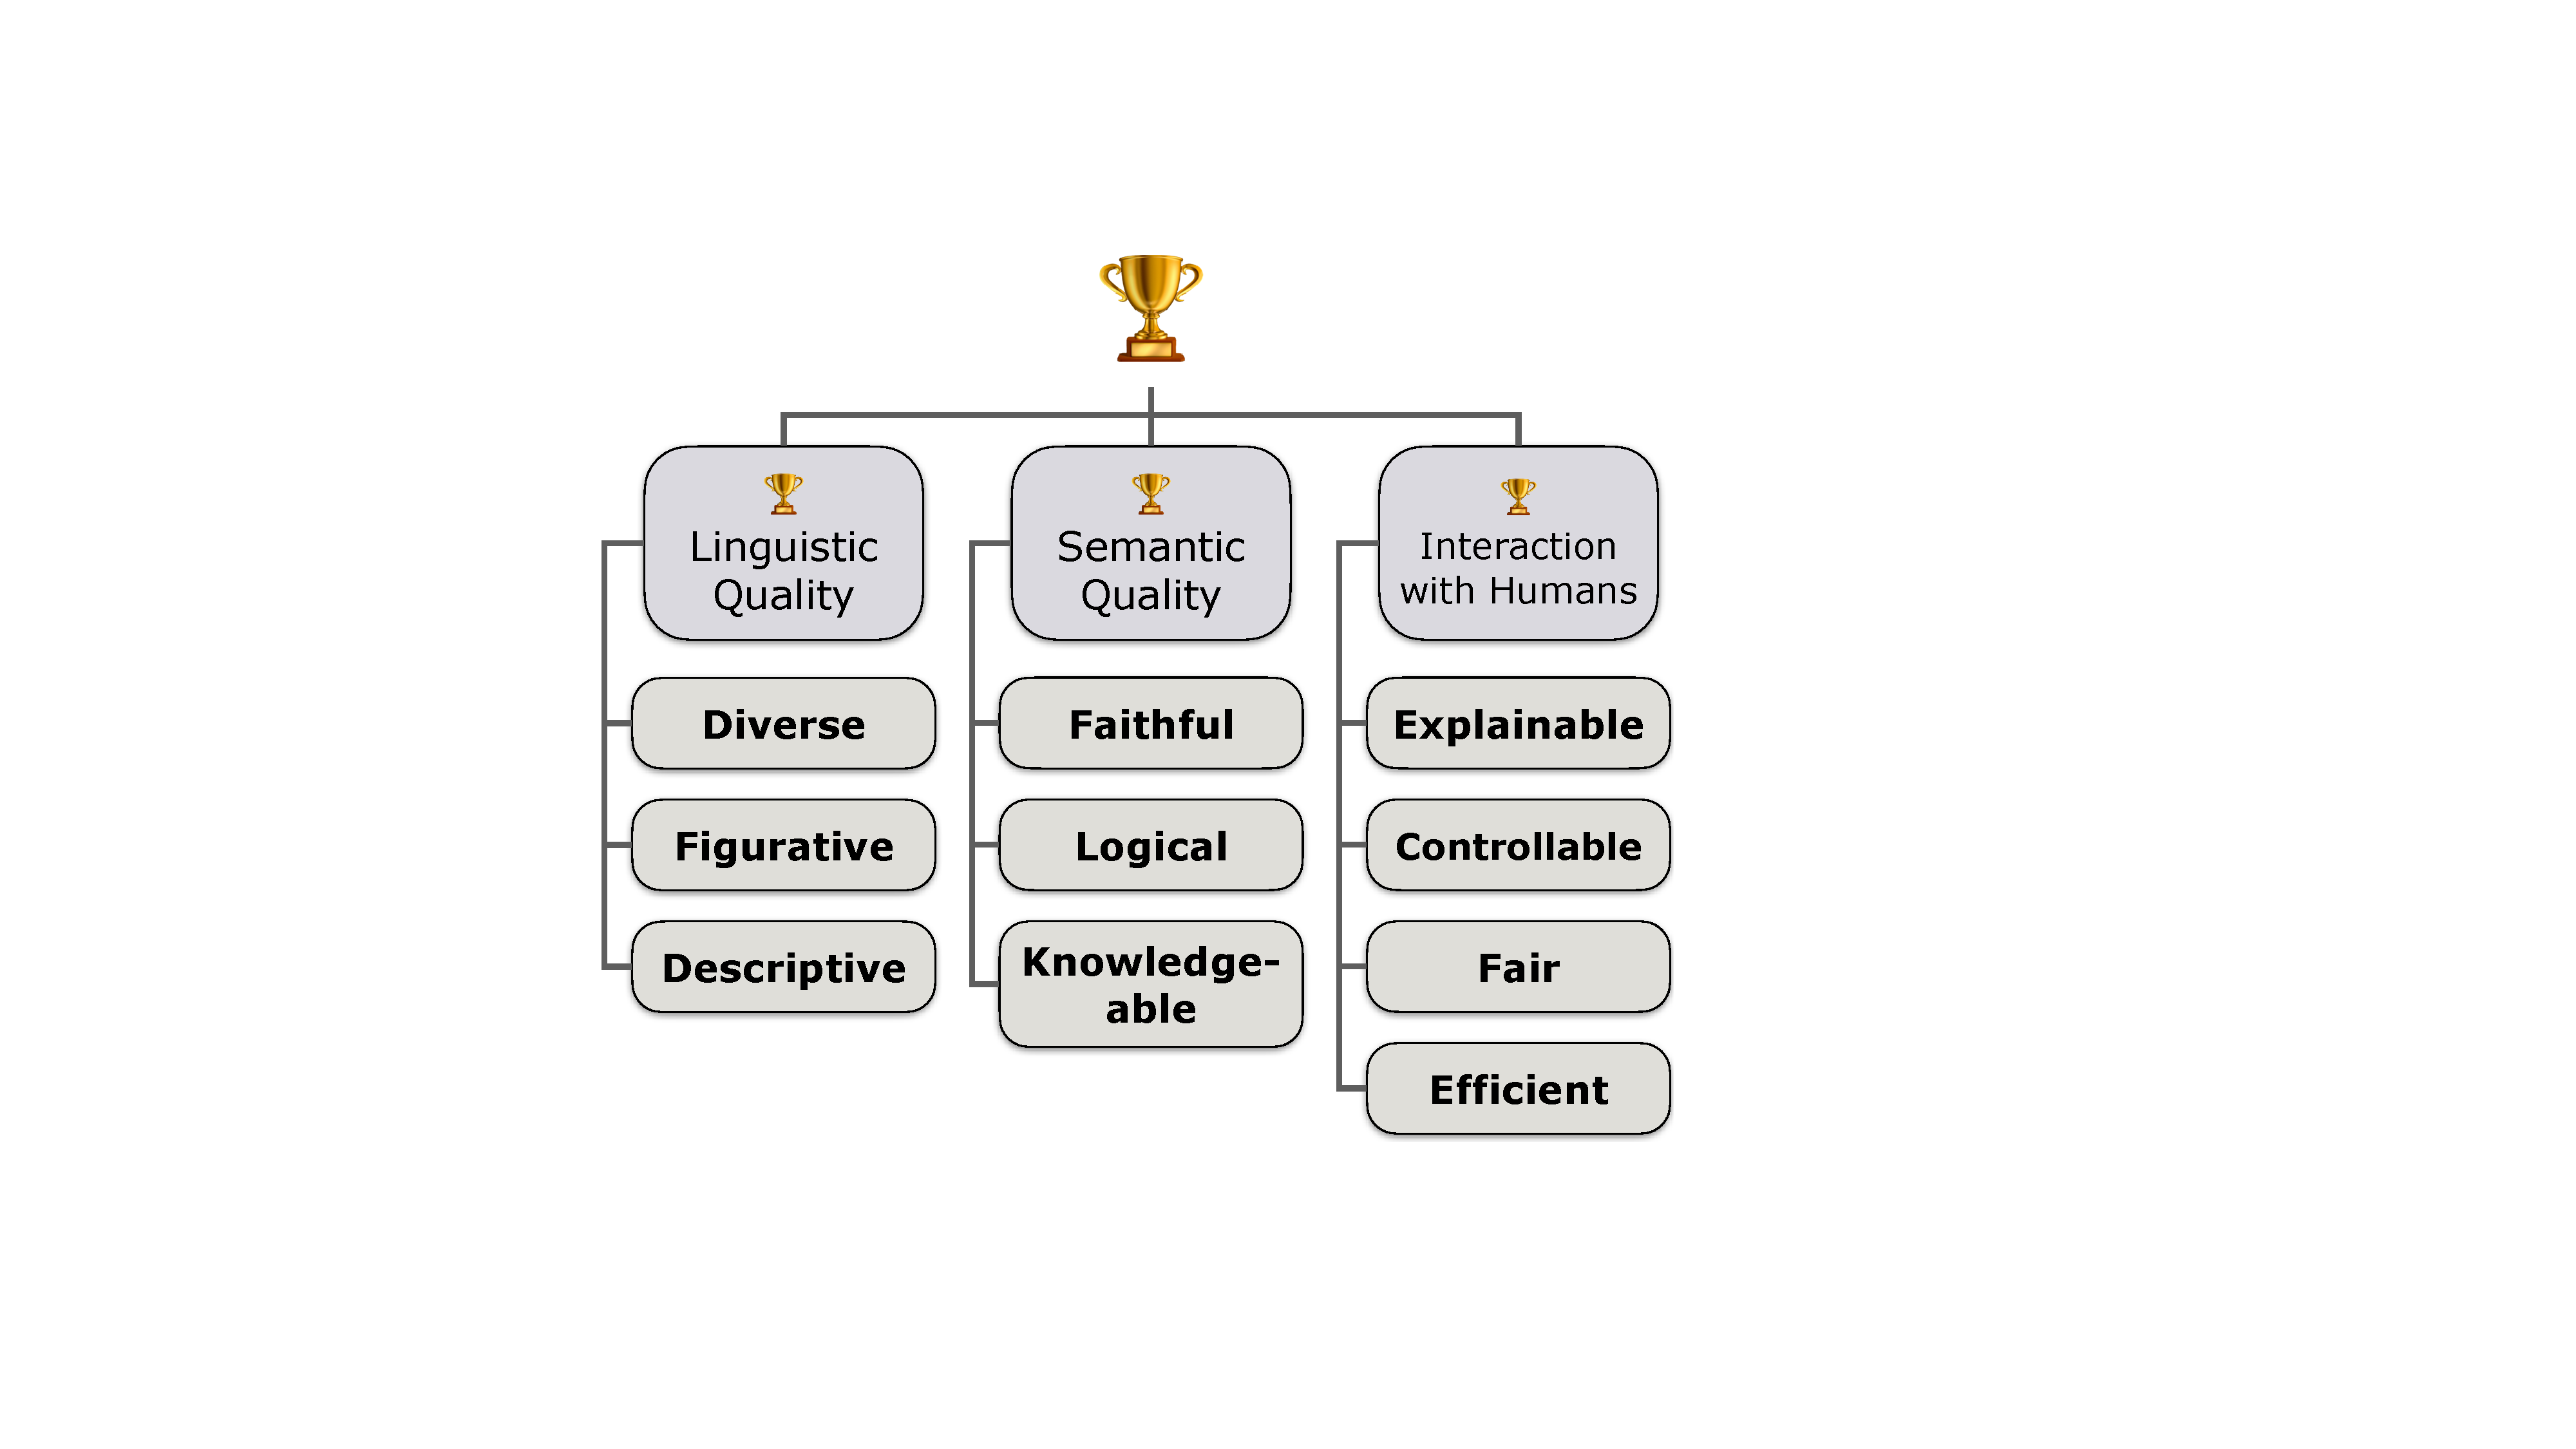
\includegraphics[width=7.5cm]{submissions/reasoning-nlp/figs/taxonomy.pdf}
    \caption{The taxonomy of the goals in NLG.}
    \label{fig:taxonomy}
\end{figure}


\paragraph{Diverse}


Given a source input, an ideal NLG model needs to be able to generate multiple and diverse outputs, where each of them needs to be equally valid.
For example
Diversified NLG is a practical goal, especially in the context of real-life applications such as dialogue generation~\cite{wu-etal-2020-diverse}, machine translation~\cite{shen2019mixture}, headline or query generation in e-commerce~\cite{10.1145/3488560.3498431} and text paraphrasing~\cite{10.1007/978-3-030-88480-2_28}.
Advanced NLG models should be able to generate diverse but informative text from the large sentence space, especially involving diverse but relevant background knowledge in the context.

\paragraph{Figurative}

The generative text should be figurative to build up emotional significance to the readers.
Figurative text typically includes idioms, sarcasm, simile, metaphor, etc.
All of them are great ingredients in interesting and creative writing tasks such as story generation or narratives.
For example, the sentence that ``he is drowning in a sea of grief'' expresses strong negative emotions to the reader, where \textit{grief}, with the metaphor of a \textit{sea}, vividly overwhelms \textit{him}.
To master the ability to write figurative text is non-trivial, and recent studies show that even strong modern language models still struggle at this objective~\cite{he-etal-2022-pre,liu-etal-2022-testing,chen-etal-2022-e}.
Nevertheless, research shows that such a problem can be alleviated with knowledge-enhanced models, which enrich the context and constituents of figurative text with acquired knowledge~\cite{chakrabarty-etal-2022-rocket}.


\paragraph{Descriptive}

Advanced NLG techniques need to be descriptive, that is, vivid and colorful as if something is being experienced by the readers.
Descriptive texts are rather common in books and novels, fascinated by image-like texts.
For example, to describe the sunset: ``\textit{the sunset filled the entire sky with the deep color of rubies, setting the clouds ablaze.}''\footnote{
https://rescuewriting.org/featured/writing-descriptive-text/.}
It is worth noting that, unlike previous desired properties that interact mostly with textual data, a system needs to integrate multi-modal knowledge and reasoning (e.g., image, video, etc.) to be descriptive with visual-specific features ~\cite{yin-ordonez-2017-obj2text,DBLP:conf/ai/Shi0Z21,shi-etal-2021-enhancing}.
However, the exact definition of descriptiveness in the context of the machine-generated text as well as its automatic evaluation are still great challenges.



\paragraph{Faithful}

The generated text should be faithful to the input so that it correctly conveys and extends the input information without semantic violation.
Otherwise, the credibility of an NLG system could be undermined when hallucinated texts are generated, which could be dangerous sometimes.
There is a growing interest in enhancing and evaluating the (intrinsic or extrinsic) faithfulness of generated text in text summarization~\cite{cao2018faithful,maynez-etal-2020-faithfulness,ladhak-etal-2022-faithful}, dialogue systems~\cite{honovich-etal-2021-q2}, text simplification~\cite{devaraj-etal-2022-evaluating}, etc.
However, hallucinated texts are not always non-factual, because they may be faithful towards world knowledge~\cite{cao-etal-2022-hallucinated}.
Therefore, an NLG system should be faithful and can be verified by world knowledge~\cite{thorne-etal-2018-fever,Chen_Bao_Sun_Zhang_Chen_Zhou_Xiao_Li_2022}, except for applications such as fictional story generation.



\paragraph{Logical}

Logical reasoning is an essential part of human thinking and language; therefore, the generated text needs to be logically consistent and self-contained.
Different from faithfulness which focuses on information consistency, logical consistency poses a challenge over the discourse of produced language of an NLG system~\cite{betz-etal-2021-critical,chen-etal-2020-logical,shi-etal-2021-refine-imitate,shu-etal-2021-logic,pi2022logigan}.
However, the training objectives of current prevailing language modeling (e.g., masked language modeling and causal language modeling) prioritize recovering given text, which does not guarantee the logical reasoning ability to be effectively captured by models.


\paragraph{Knowledgeable}

An NLG model needs to be knowledgeable to generate text that is rich in knowledge~\cite{yu2022survey}.
When engaging in a conversation, current NLG models are known to be dependent on plain but safe responses.
A knowledgeable NLG system, in contrast, should be able to actively initiate responses grounded with the background knowledge that is either retrieved~\cite{NEURIPS2020_6b493230} or inherent~\cite{liu-etal-2022-multi} in the system itself.
Also, it is worth exploring whether current NLG models are using knowledge of their own or just relying on statistical patterns learned from (pre-)training~\cite{cao-etal-2021-knowledgeable}.


\paragraph{Explainable}
An NLG system should be explainable for the trust of human users.
Since language is the most natural tool for communication, the reasoning and decisions of a model should be explanatory through generated language~\cite{reiter2019natural}.
Existing work usually focuses on generating natural language explanations~\cite{wiegreffe-marasovic-2021-review} as a task, while how to develop universal explanation generators~\cite{ye2022unreliability} is still challenging.
More importantly, unlike natural language understanding models (NLU)~\cite{lime,Schulz2020Restricting,10.5555/3305890.3306024}, the explainability of NLG systems is severely underexplored.



\paragraph{Controllable}

Controllable NLG aims to generate with desired attributes by users, which greatly broadens its applications.
Current commonly used attributes focus on discriminative attributes such as sentiment and style, lexical constraints, and various properties of language such as lengths or complexity~\cite{NEURIPS2021_d0f5edad,zhang2022survey,garbacea2022constrained}.
Moreover, there are still many interesting open questions for building an ideal NLG system, for example, more diverse applications of controlling factors, satisfying multiple types of constrained attributes (perhaps a mixture of them), and being controlled in a few-shot or even zero-shot manner.
It is worth noting that recent studies in large language models~\cite{NEURIPS2020_1457c0d6} shed some light on these research problems.


\paragraph{Fair}

The generated text should be fair and contain no bias whatsoever.
Methods to mitigate biases have been proposed w.r.t. gender, race, nationality, age, disability, religion, etc.
\cite{liu-etal-2020-gender,xia-etal-2020-demoting,gupta-etal-2022-mitigating}.
Since text generation models have been widely applied in the age of the Internet, their outstanding performance could blind service providers so as to omit the negative social impacts that an unfair NLG system causes.
However, since modern NLG systems are usually pre-trained on colossal unannotated corpus~\cite{radford2019language,raffel2020exploring,lewis-etal-2020-bart,NEURIPS2020_1457c0d6}, the biases within them are still rather difficult to eliminate.



\paragraph{Efficient}

An NLG system should be efficient to be deployed on high-demanding scenarios such as mobile devices or online industrial applications.
Recent work on non-autoregressive generation (NAG)~\cite{gu2018nonautoregressive,xiao2022survey}, which generates tokens in parallel, has shown promising potential in efficiency.
This enables NAG to achieve over $10\times$ speedup over the autoregressive counterpart (AG) that generates in a left-to-right manner~\cite{vaswani2017attention}.
However, NAG is still haunted by the multi-modality problem~\cite{Zhou2020Understanding}, its generality to tasks other than machine translation~\cite{qian-etal-2021-glancing}, and interaction with external knowledge~\cite{zeng-etal-2022-neighbors}.


\section{Knowledge in Language Generation}
\label{sec:knowledge}
%[TODO: add a figure: knowledge-generation interaction]


In this section, we briefly review some representative work in knowledge-guided NLG algorithms and knowledge acquisition with NLG models, where NLG systems also show unique advantages in the latter.
Figure~\ref{fig:knowledge-nlg} shows the relation between knowledge-guided NLG ($\mathsection$~\ref{subsec:knowledge-guided-nlg}) and knowledge acquisition with NLG ($\mathsection$~\ref{subsec:generative_acquisition}), where the two are mutually beneficial to each other.

\begin{figure}[tp]
    \centering
    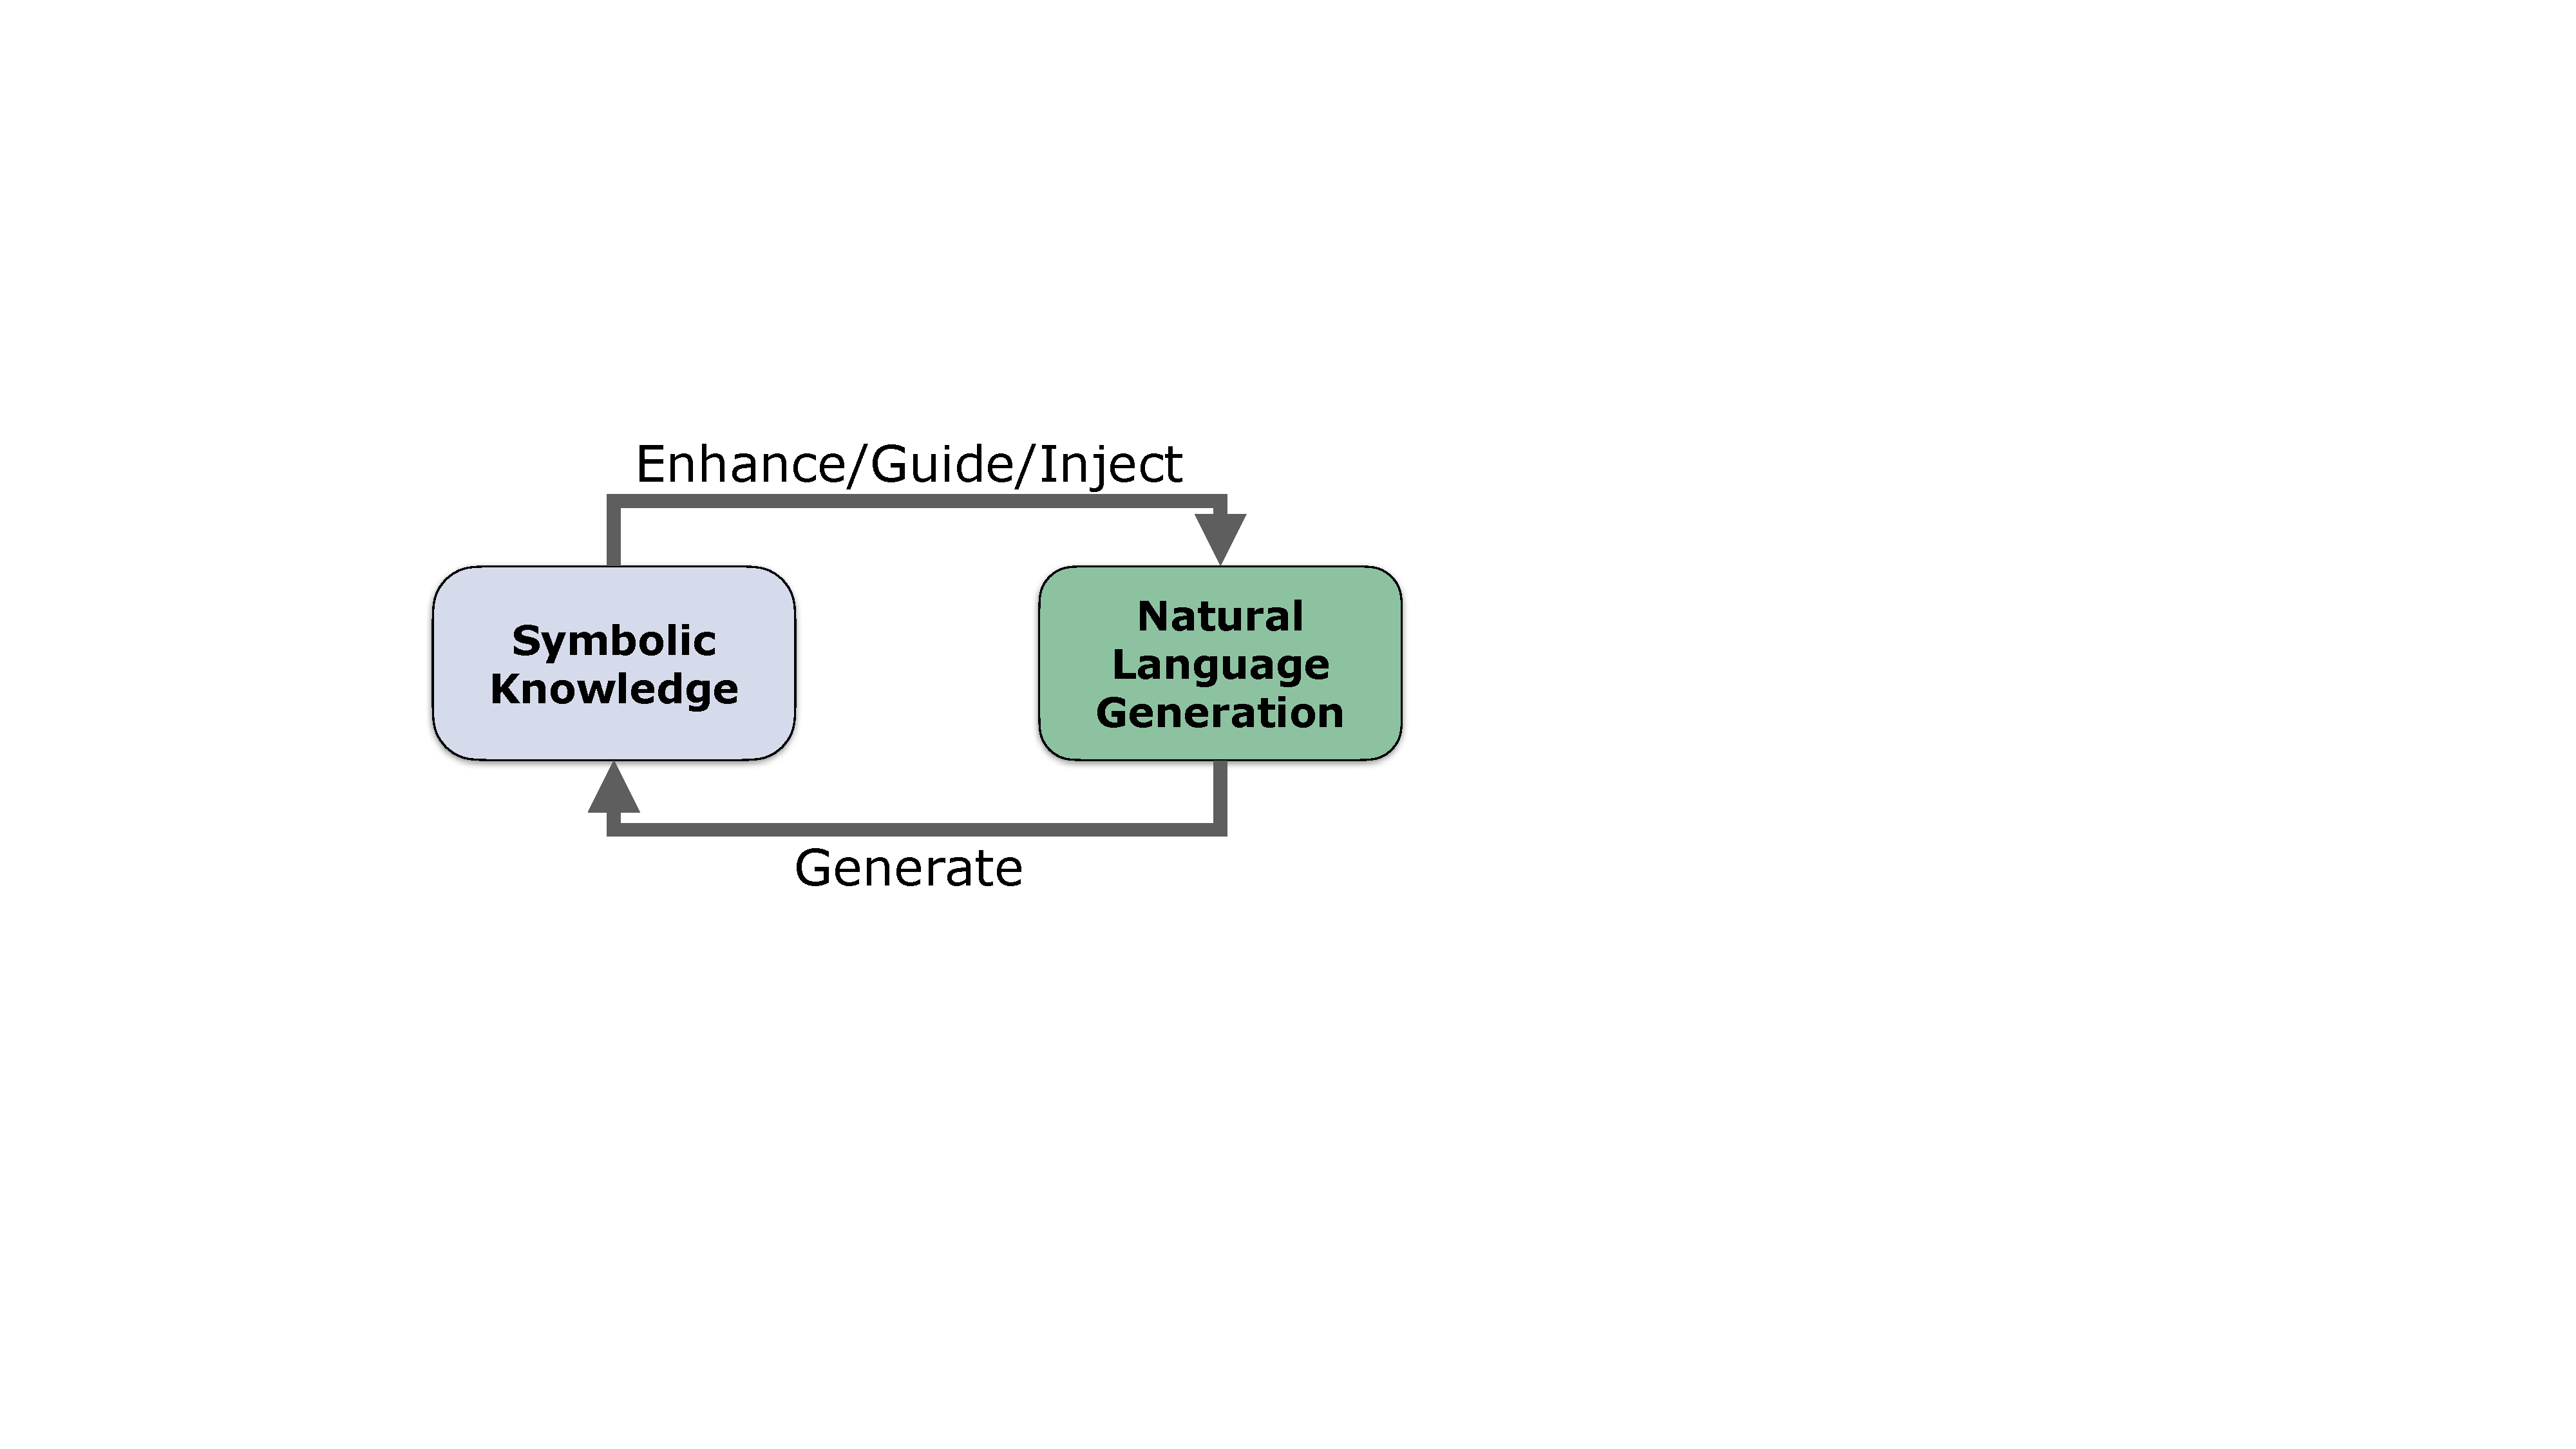
\includegraphics[width=7.5cm]{submissions/reasoning-nlp/figs/knowledge-nlg.pdf}
    \caption{Relations between knowledge and NLG, where knowledge can enhance, guide and be injected into NLG systems, and NLG systems can be utilized as tools to generate new knowledge.}
    \label{fig:knowledge-nlg}
\end{figure}

\subsection{Knowledge-guided NLG: Tricks of the Trade}
\label{subsec:knowledge-guided-nlg}

NLG systems can be guided by multiple sources and types of knowledge to be logical, diverse, faithful, controllable, etc.
In the following text, we list the knowledge sources that are commonly used, and showcase the common tricks of current knowledge-guided NLG algorithms, presenting a brief but as comprehensive review as possible.

\paragraph{Knowledge Sources}

According to Yu et al. \cite{yu2022survey}, knowledge sources used in NLG systems can be categorized into internal and external knowledge, where:
1) internal knowledge is created within the given text, e.g., keywords, topics, linguistic features, etc.,
and 2) external knowledge exists outside the input of the NLG system, e.g., knowledge bases/graphs, grounded unstructured text.
We add that knowledge mined from the corpus is also important to guide NLG systems, such as concepts, rules, and patterns~\cite{chen-etal-2019-ensuring}.
Notably, NLG systems form an interesting dual learning loop where knowledge can be acquired by NLG systems ($\mathsection$ \ref{subsec:generative_acquisition}) and used in NLG systems~\cite{sun-etal-2018-logician,cao-etal-2020-unsupervised-dual}.
Next, we will detail some common practices of NLG models that involve knowledge.

\paragraph{Knowledge Incorporation in Model Architectures}
Modifying model architectures to incorporate knowledge is one of the most commonly used approaches in knowledge-guided NLG~\cite{yang2021survey,yu2022survey}.
Typical methods include using attention mechanism~\cite{DBLP:journals/corr/BahdanauCB14} (and its variants, e.g., copying mechanism,~\cite{gu-etal-2016-incorporating}) to attend additional knowledge sources, encoding knowledge with specific encoders (e.g., graph neural networks,~\cite{kipf2016semi}), adding specific layers in the neural network for knowledge storage (e.g., adapter layers,~\cite{guo2020incorporating}), etc.
In this line of work, a model trains to utilize the encoded knowledge for better NLG.
However, such methods usually require the design of an ad hoc model architecture, which does not generalize well to new tasks, especially in the age of large PLMs~\cite{NEURIPS2020_1457c0d6}.


\paragraph{Learning with Knowledge}

The most common method of knowledge-guided NLG is through supervised learning, where the guidance of knowledge can be well integrated into generation~\cite{yu2022survey}.
A simple way to do this is to append the acquired knowledge to the input as an additional context.
This has been shown to be effective, especially when knowledge acquisition (e.g., retrieval) is jointly trained with generation~\cite{pmlr-v119-guu20a,NEURIPS2020_6b493230}.
Another way is to guide learning objectives with knowledge.
Studies in this direction are carried out by designing knowledge into one of the training targets~\cite{cao-etal-2020-unsupervised-dual} or pre-training~\cite{guan-etal-2020-knowledge}, or by introducing additional knowledge-related objective functions to regularize training~\cite{hu2018deep}.
Also, reward design in a reinforcement learning (RL) framework is a flexible way of integrating knowledge into training objectives for NLG models.
For an example of improving the consistency between source and target, \cite{li2018ensure} injects the entailment knowledge into NLG with an entailment model, and \cite{huang-etal-2020-knowledge} designs a semantic cloze reward for faithful summarization.

\paragraph{Knowledge-Constrained Decoding}

Finally, we would like to emphasize knowledge incorporation during decoding.
Knowledge injection through model architecture modification and new learning objectives, despite being effective, requires (re-)training.
This usually causes inconvenience for deployment, especially with large PLMs.
For this reason, constraining text decoding in inference time with knowledge has become a promising research topic~\cite{zhang2022survey,garbacea2022constrained}.
In this line of work, we briefly introduce the three most exemplary knowledge constraint types in NLG systems:
1) lexical knowledge constraints, such as keywords that must appear in the text,
2) discriminative constraints, such as the desired attributes of the generated text, and
3) structured knowledge constraints, such as the world knowledge that the generated text must be consistent with.



Imposing \textit{lexical constraints} is challenging for NLG systems because the prevailing ones usually generate in an autoregressive manner, which is difficult to know when and where to keep the constraints.
Popular solutions to this problem mainly focus on adding constraints during beam search~\cite{hokamp-liu-2017-lexically,post-vilar-2018-fast,lu-etal-2021-neurologic} at the cost of computational complexity.
Recent work~\cite{susanto-etal-2020-lexically,10.1162/tacl_a_00368} also explores iterative lexically constrained decoding for non-autoregressive models, achieving significant speedups.

\textit{Discriminative constraints} usually involve prior attribute models to control the generated text in terms of attributes such as topics (sport, finance, medical), sentiments (positive, negative), etc.
Exemplary work is PPLM ~\cite{Dathathri2020Plug}, which controls the attribute of generated text without changing the parameters of the backbone PLM (e.g., GPT-2,~\cite{radford2019language}).
During sampling, PPLMs back-propagates the gradient from the attribute model to the hidden states of the PLM so that the generation can be steered by the attribute model.
Under such a framework, it is easy to guide generation with prior knowledge.
It is worth noting that work on text sampling is also a great framework to effectively incorporate the above-mentioned two types of constraints.
In this framework, the desired properties are designed as objective functions, guiding the sampling process, which is usually instantiated with Markov chain Monte Carlo methods~\cite{Miao_Zhou_Mou_Yan_Li_2019,zhang-etal-2020-language-generation,qin2022cold}.
Similar to PPLM, such methods ensure the generated text is constrained to the desired objectives without training.


Recent studies have also started to pay attention to the hallucination problem of NLG systems (represented by PLMs) from the perspective of constrained decoding with \textit{structured knowledge constraints}, such as knowledge graphs.
For example, \cite{liu2022knowledge} retrieves from knowledge graphs related to neighboring entities within source input.
They are used to modify and constrain the distributions over the vocabulary during sampling, where tokens within knowledge graphs are rewarded.
In this way, the generated text would be rich in semantic knowledge and faithful to world knowledge, making it an interesting and effective solution to the hallucination problem that is common in NLG.


% Sampling-based NLG models, due to its flexibility, are also great frameworks to effectively incorporate the above-mentioned constraints.
%~\cite{Miao_Zhou_Mou_Yan_Li_2019}
%~\cite{zhang-etal-2020-language-generation}
%~\cite{qin2022cold}

\subsection{Knowledge Acquisition with NLG}
\label{subsec:generative_acquisition}
Knowledge acquisition based on NLG systems aims to generate knowledge from the input text.
Compared with other paradigms of knowledge acquisition, automatic and generalizability to unseen knowledge are one of the most desired features of generative methods.
In the following text, we first discuss current knowledge acquisition paradigms and show the advantages of generative methods in certain scenarios.

\paragraph{Paradigms of Knowledge Acquisition}

The knowledge acquisition methods can be divided into three categories: 1) crowd-sourcing, 2) extractive and 3) generative methods.
The \textit{crowd-sourcing} methods~\cite{10.1145/219717.219748} invite some experts to label the knowledge in the corpus, which can acquire accurate knowledge but only have a small size due to costly annotation.
The \textit{extractive} methods~\cite{zhou2022survey} adopt language models to extract the knowledge explicitly mentioned in the input text automatically but ignore some symbolic and neural commonsense knowledge.
Compared with them, generative knowledge acquisition methods enjoy the advantages of the ability to generate explicit and implicit knowledge, which we will soon discuss.


\paragraph{Meta Knowledge Generation}
Meta knowledge is knowledge about knowledge~\cite{Davis1977MetaLevelKO}.
As a fundamental conceptual instrument in knowledge-based domains, meta-knowledge can greatly improve the performance of downstream tasks, such as text classification~\cite{chen2019deep}, question answering~\cite{garderes-etal-2020-conceptbert} and story generation~\cite{chen2021commonsense}.
However, meta-knowledge is hardly explicitly mentioned in the corpus, and thus it is difficult to directly extract meta-knowledge from the text.
Alternatively, since NLG systems can generate information never mentioned in the text and has a strong generalization ability of unseen knowledge, recent work proposes to adopt generative methods to acquire meta knowledge, such as concepts~\cite{chen-etal-2019-ensuring,9409694} and rules~\cite{10.1016/j.knosys.2022.108371}.

\paragraph{Generative Knowledge Retrieval}
Information retrieval aims to retrieve meaningful information from large Knowledge Bases (KB) given a textual input.
Compared to extractive methods, generative information retrieval~\cite{cao2021autoregressive,10.1162/tacl_a_00460,rossiello2021generative} can directly capture the relation between context and target information and reduce the memory footprint without negative data down-sampling.

\paragraph{Generative Knowledge Extraction}
Information extraction aims to obtain information from semi-structured and unstructured text, which suffers heterogeneous structures and domain-specific schemas~\cite{lu-etal-2022-unified}.
The generative information extraction can end-to-end generate targeted structures directly.
For example, \cite{huguet-cabot-navigli-2021-rebel-relation} adopts autoregressive models to achieve the extraction of end-to-end relations.
\cite{lu-etal-2021-text2event} proposes a sequence-to-structure generation method to directly extract events from the text.
\cite{huang-etal-2021-document} formulates entity-based extraction as a template generation task to allow the generative framework to effectively capture cross-entity dependencies.


\paragraph{Knowledge Generation}

NLG models can also be used for the completion of knowledge bases, including commonsense knowledge graphs and rules.
Instead of extracting semi-structured and unstructured text into knowledge, some work~\cite{bosselut-etal-2019-comet,Hwang2021COMETATOMIC2O} feeds large-scale language models with a massive corpus to obtain knowledge models, which can adapt their learned representations to knowledge generation and automatically construct KBs.
Furthermore, the parameters of PLMs are shown to store vast amounts of linguistic knowledge~\cite{47786}.
A line of work further regards PLMs as knowledge bases and distills semantic knowledge from these models~\cite{petroni-etal-2019-language,alkhamissi2022review}.



\section{Reasoning in Language Generation}
\label{sec:reasoning}

We echo the argument that good reasoning should be right for the right reasons.
Therefore, it is also crucial for an NLG model to make \textit{rational} usage of knowledge to approach human-like reasoning skills.
This section signifies the importance of reasoning in NLG, where we sketch two lines of research: 1) reasoning-guided NLG methods ($\mathsection$~\ref{subsec:reasoning-guided-nlg}) and 2) NLG for the purpose of reasoning ($\mathsection$~\ref{subsec:reasoning-by-nlg}).



\subsection{Reasoning-guided NLG}
\label{subsec:reasoning-guided-nlg}
In contrast to general knowledge-guided NLG, reasoning-guided NLG systems make more rational and explainable usage of the knowledge (in wide forms).
Since reasoning is highly correlated with knowledge ($\mathsection$ \ref{sec:knowledge}), we will discuss reasoning-guided NLG by highlighting the topics of graph reasoning and generative reasoning tasks in the following paragraphs.

\paragraph{Graph Reasoning}

Graph reasoning is one of the most commonly used techniques to guide NLP systems towards more multihop, controllable, and explainable reasoning.
Therefore, we extend what has been discussed in $\mathsection$ \ref{subsec:knowledge-guided-nlg} in this paragraph for introducing graph reasoning-guided NLG.
Graph reasoning implementations are usually built on retrieved subgraphs of external knowledge graphs~\cite{Liu_Wan_He_Peng_Yu_2021} or internal graphs parsed from the input~\cite{wang-etal-2020-heterogeneous}.
Most of them adopt graph embeddings~\cite{NIPS2013_1cecc7a7} and graph neural networks~\cite{kipf2016semi,velickovic2018graph} to propagate information throughout the graph.
These properties of graphs enable the multi-hop reasoning ability of NLG models for long-range text~\cite{ji-etal-2020-language} and generating emerging concepts or topics guided by the graph~\cite{wang-etal-2019-paperrobot,zhang-etal-2020-grounded}.
Due to the symbolic structure of graphs, heuristics and prior knowledge can be easily incorporated into graph construction, e.g., building graphs with various parsing tools ~\cite{gardner2017allennlp} such as semantic role labeling or dependency parsing or guiding graph propagation with more information, such as popularity knowledge~\cite{10.1145/3488560.3498431}.
Also, such methods are explainable and easy to debug, since the weights on the graph nodes and edges greatly facilitate post hoc manual examination.


\paragraph{Reasoning Tasks}

One of the most direct ways to enable NLG models to reason is to design various reasoning tasks.
During the solving of these tasks, researchers can develop and test their models w.r.t. corresponding reasoning skills, which makes it an important direction to guide AI models.
Over the years, the community has accumulated many datasets of tasks that test various facets of machine reasoning in the form of text generation.
Most of them are built from the point of view of human cognition, including tasks about logical reasoning~\cite{dalvi-etal-2021-explaining}, abductive reasoning~\cite{bhagavatula2020abductive}, counterfactual reasoning~\cite{qin-etal-2019-counterfactual}, generative commonsense reasoning~\cite{lin-etal-2020-commongen}, social reasoning~\cite{sap-etal-2019-social}, physical reasoning~\cite{Bisk_Zellers_Le_bras_Gao_Choi_2020}, temporal reasoning~\cite{zhou-etal-2019-going}, etc. \footnote{Note that some of these reasoning tasks~\cite{sap-etal-2019-social,Bisk_Zellers_Le_bras_Gao_Choi_2020,zhou-etal-2019-going} take the form of question answering but can be solved in a generative manner~\cite{2020unifiedqa}.}
Not limited to these tasks, datasets on explanation generation~\cite{wiegreffe-marasovic-2021-review} are also good sources to evaluate and improve the reasoning ability of NLG systems, including the explanations for natural language inference~\cite{NEURIPS2018_4c7a167b} commonsense reasoning~\cite{rajani-etal-2019-explain}, analogical reasoning~\cite{chen-etal-2022-e}, causal reasoning~\cite{du-etal-2022-e}, multimodal reasoning~\cite{li2018vqae}, etc.


%~\cite{bhargava2022commonsense}

% Their dataset contains arguments each with a claim, an explicit premise, and two implicit warrants.
% The objective is to choose the correct warrant that forms the deductive argument.

% Abductive reasoning aims at generating the best possible explanation for a reasoning process.
% It focuses on filling the gap between an observation (or premise) and a conclusion.


% Counterfactual reasoning.
%~\cite{chen2021unsupervised}

\subsection{Reasoning by NLG}
\label{subsec:reasoning-by-nlg}

Human language is a good vehicle for reasoning.
Thus, the generation of language naturally resembles the way humans think and reason.
With the success of PLMs, there is a growing interest in the AI community to use NLG models to generate a chain of reasoning for problem-solving.


\paragraph{Generative Reasoning}


Generative reasoning aims to generate intermediate reasons with NLG models for better problem solving.
Such intermediate reasons take many forms, including deduction and abduction reasons~\cite{tafjord-etal-2021-proofwriter},  explanations~\cite{jhamtani-clark-2020-learning}, or decomposed subtasks of a complex one~\cite{khot-etal-2021-text}.
Some work~\cite{shwartz-etal-2020-unsupervised,betz2021thinking} even show that expanding the context of the input by generating more information would also help solve reasoning tasks.
Moreover, \cite{ijcai2020-0537} finds that transformer-based PLMs are effective soft reasoners on a toy deduction dataset, which consists of collections of text verbalized from artificial if-then rules and facts.
Other studies~\cite{bostrom-etal-2021-flexible,betz-etal-2021-critical} corroborate this discovery and show that training generative models with artificial textual data that verbalize rule-based reasoning helps downstream logical reasoning tasks.
We remark that generative reasoning provides a new perspective of breaking the black-box prediction of neural networks, which demonstrates the potential of achieving reasoning with NLG systems.



\paragraph{Reasoning with Large Language Models}

Entering the era of large language models (LLMs) such as GPT-3~\cite{NEURIPS2020_1457c0d6,ouyang2022training} and PaLM~\cite{chowdhery2022palm}, there is a recent growing interest in exploring few-/zero-shot reasoning skills of these LLMs
Since fine-tuning such tremendous language models is hardly possible, current work adopts prompt-based in-context learning methods~\cite{NEURIPS2020_1457c0d6,lu-etal-2022-fantastically} to achieve few-/zero-shot learning with LLMs, where instructions and examples are demonstrated within the input prompts.


Similar to the above discussion of generative reasoning, this line of work aims to guide the language models to explicitly generate the intermediate thinking steps (or reasons) during reasoning.
A representative work among them is the Chain-of-Thought prompting~\cite{wei2022chain}, where the intermediate thinking process is verbalized and integrated into the demonstrations.
In this way, complex reasoning can be decomposed into multiple steps reflected by language, which is analogous to how humans solve complex tasks.
Such methods achieve much better performance on a variety of reasoning tasks compared with normal prompting and even surpass fine-tuned methods in some cases.
Moreover, the prompting strategy can be further refined~\cite{wang2022self,zhou2022least,creswell2022selection}, leading to generally better results.
LLMs prompted with and asked to generate step-by-step reasoning chains also exhibit certain quantitative reasoning abilities such as solving math word problems~\cite{wei2022chain}, where the LLMs are not specifically trained on such tasks.
However, reasoning abilities for LLMs are shown to be emergent~\cite{wei2022chain,wei2022emergent}, i.e., effective only for really large language models (over 100 billion parameters).
How to enable smaller language models with few-shot reasoning skills is still an open question.


\section{Conclusion}
\label{sec:conclusion}

In this work, we envision the ten most desired goals of an intelligent natural language generation system.
In pursuit of these goals, the guidance of knowledge and reasoning plays a significant role in modern NLG models.
We have revisited the achievements with knowledge in NLG w.r.t. knowledge-guided NLG and generative knowledge acquisition.
We particularly highlight knowledge-constrained decoding for its wide application potential, where knowledge constraints can be incorporated into NLG models (especially large-scale ones) in a plug-and-play manner.
We have also discussed current work on reasoning in NLG, which essentially makes rational usage of knowledge and datasets for various reasoning tasks.
Moreover, NLG can verbalize intermediate thinking processes to facilitate complex reasoning, enabling few-/zero-shot reasoning abilities for large language models.
However, current research is still far from realizing these goals, which we outline for future research.
We hope that this survey report can provide newcomers with a good entry point into the exciting area of knowledge-guided and reasoning-intensive NLG.


%\bibliographystyle{plain}
%\bibliography{submissions/reasoning-nlp/custom}

\begin{thebibliography}{100}

\bibitem{alkhamissi2022review}
Badr AlKhamissi, Millicent Li, Asli Celikyilmaz, Mona Diab, and Marjan
  Ghazvininejad.
\newblock A review on language models as knowledge bases.
\newblock {\em arXiv preprint arXiv:2204.06031}, 2022.

\bibitem{10.5555/1785162.1785216}
S\"{o}ren Auer, Christian Bizer, Georgi Kobilarov, Jens Lehmann, Richard
  Cyganiak, and Zachary Ives.
\newblock Dbpedia: A nucleus for a web of open data.
\newblock In {\em Proceedings of the 6th International The Semantic Web and 2nd
  Asian Conference on Asian Semantic Web Conference}, ISWC'07/ASWC'07, page
  722–735, Berlin, Heidelberg, 2007. Springer-Verlag.

\bibitem{DBLP:journals/corr/BahdanauCB14}
Dzmitry Bahdanau, Kyunghyun Cho, and Yoshua Bengio.
\newblock Neural machine translation by jointly learning to align and
  translate.
\newblock In Yoshua Bengio and Yann LeCun, editors, {\em 3rd International
  Conference on Learning Representations, {ICLR} 2015, San Diego, CA, USA, May
  7-9, 2015, Conference Track Proceedings}, 2015.

\bibitem{betz2021thinking}
Gregor Betz, Kyle Richardson, and Christian Voigt.
\newblock Thinking aloud: Dynamic context generation improves zero-shot
  reasoning performance of gpt-2.
\newblock {\em arXiv preprint arXiv:2103.13033}, 2021.

\bibitem{betz-etal-2021-critical}
Gregor Betz, Christian Voigt, and Kyle Richardson.
\newblock Critical thinking for language models.
\newblock In {\em Proceedings of the 14th International Conference on
  Computational Semantics (IWCS)}, pages 63--75, Groningen, The Netherlands
  (online), June 2021. Association for Computational Linguistics.

\bibitem{bhagavatula2020abductive}
Chandra Bhagavatula, Ronan~Le Bras, Chaitanya Malaviya, Keisuke Sakaguchi, Ari
  Holtzman, Hannah Rashkin, Doug Downey, Wen tau Yih, and Yejin Choi.
\newblock Abductive commonsense reasoning.
\newblock In {\em International Conference on Learning Representations}, 2020.

\bibitem{Bisk_Zellers_Le_bras_Gao_Choi_2020}
Yonatan Bisk, Rowan Zellers, Ronan Le~bras, Jianfeng Gao, and Yejin Choi.
\newblock Piqa: Reasoning about physical commonsense in natural language.
\newblock {\em Proceedings of the AAAI Conference on Artificial Intelligence},
  34(05):7432--7439, Apr. 2020.

\bibitem{NIPS2013_1cecc7a7}
Antoine Bordes, Nicolas Usunier, Alberto Garcia-Duran, Jason Weston, and Oksana
  Yakhnenko.
\newblock Translating embeddings for modeling multi-relational data.
\newblock In C.J. Burges, L.~Bottou, M.~Welling, Z.~Ghahramani, and K.Q.
  Weinberger, editors, {\em Advances in Neural Information Processing Systems},
  volume~26. Curran Associates, Inc., 2013.

\bibitem{bosselut-etal-2019-comet}
Antoine Bosselut, Hannah Rashkin, Maarten Sap, Chaitanya Malaviya, Asli
  Celikyilmaz, and Yejin Choi.
\newblock {COMET}: Commonsense transformers for automatic knowledge graph
  construction.
\newblock In {\em Proceedings of the 57th Annual Meeting of the Association for
  Computational Linguistics}, pages 4762--4779, Florence, Italy, July 2019.
  Association for Computational Linguistics.

\bibitem{bostrom-etal-2021-flexible}
Kaj Bostrom, Xinyu Zhao, Swarat Chaudhuri, and Greg Durrett.
\newblock Flexible generation of natural language deductions.
\newblock In {\em Proceedings of the 2021 Conference on Empirical Methods in
  Natural Language Processing}, pages 6266--6278, Online and Punta Cana,
  Dominican Republic, November 2021. Association for Computational Linguistics.

\bibitem{NEURIPS2020_1457c0d6}
Tom Brown, Benjamin Mann, Nick Ryder, Melanie Subbiah, Jared~D Kaplan, Prafulla
  Dhariwal, Arvind Neelakantan, Pranav Shyam, Girish Sastry, Amanda Askell,
  Sandhini Agarwal, Ariel Herbert-Voss, Gretchen Krueger, Tom Henighan, Rewon
  Child, Aditya Ramesh, Daniel Ziegler, Jeffrey Wu, Clemens Winter, Chris
  Hesse, Mark Chen, Eric Sigler, Mateusz Litwin, Scott Gray, Benjamin Chess,
  Jack Clark, Christopher Berner, Sam McCandlish, Alec Radford, Ilya Sutskever,
  and Dario Amodei.
\newblock Language models are few-shot learners.
\newblock In H.~Larochelle, M.~Ranzato, R.~Hadsell, M.F. Balcan, and H.~Lin,
  editors, {\em Advances in Neural Information Processing Systems}, volume~33,
  pages 1877--1901. Curran Associates, Inc., 2020.

\bibitem{NEURIPS2018_4c7a167b}
Oana-Maria Camburu, Tim Rockt\"{a}schel, Thomas Lukasiewicz, and Phil Blunsom.
\newblock e-snli: Natural language inference with natural language
  explanations.
\newblock In S.~Bengio, H.~Wallach, H.~Larochelle, K.~Grauman, N.~Cesa-Bianchi,
  and R.~Garnett, editors, {\em Advances in Neural Information Processing
  Systems}, volume~31. Curran Associates, Inc., 2018.

\bibitem{cao-etal-2021-knowledgeable}
Boxi Cao, Hongyu Lin, Xianpei Han, Le~Sun, Lingyong Yan, Meng Liao, Tong Xue,
  and Jin Xu.
\newblock Knowledgeable or educated guess? revisiting language models as
  knowledge bases.
\newblock In {\em Proceedings of the 59th Annual Meeting of the Association for
  Computational Linguistics and the 11th International Joint Conference on
  Natural Language Processing (Volume 1: Long Papers)}, pages 1860--1874,
  Online, August 2021. Association for Computational Linguistics.

\bibitem{cao-etal-2022-hallucinated}
Meng Cao, Yue Dong, and Jackie Cheung.
\newblock Hallucinated but factual! inspecting the factuality of hallucinations
  in abstractive summarization.
\newblock In {\em Proceedings of the 60th Annual Meeting of the Association for
  Computational Linguistics (Volume 1: Long Papers)}, pages 3340--3354, Dublin,
  Ireland, May 2022. Association for Computational Linguistics.

\bibitem{cao2021autoregressive}
Nicola~De Cao, Gautier Izacard, Sebastian Riedel, and Fabio Petroni.
\newblock Autoregressive entity retrieval.
\newblock In {\em International Conference on Learning Representations}, 2021.

\bibitem{cao-etal-2020-unsupervised-dual}
Ruisheng Cao, Su~Zhu, Chenyu Yang, Chen Liu, Rao Ma, Yanbin Zhao, Lu~Chen, and
  Kai Yu.
\newblock Unsupervised dual paraphrasing for two-stage semantic parsing.
\newblock In {\em Proceedings of the 58th Annual Meeting of the Association for
  Computational Linguistics}, pages 6806--6817, Online, July 2020. Association
  for Computational Linguistics.

\bibitem{cao2018faithful}
Ziqiang Cao, Furu Wei, Wenjie Li, and Sujian Li.
\newblock Faithful to the original: Fact aware neural abstractive
  summarization.
\newblock In {\em Thirty-Second AAAI Conference on Artificial Intelligence},
  2018.

\bibitem{chakrabarty-etal-2022-rocket}
Tuhin Chakrabarty, Yejin Choi, and Vered Shwartz.
\newblock It{'}s not rocket science: Interpreting figurative language in
  narratives.
\newblock {\em Transactions of the Association for Computational Linguistics},
  10:589--606, 2022.

\bibitem{chen2021commonsense}
Hong Chen, Yifei Huang, Hiroya Takamura, and Hideki Nakayama.
\newblock Commonsense knowledge aware concept selection for diverse and
  informative visual storytelling.
\newblock In {\em Proceedings of the AAAI Conference on Artificial
  Intelligence}, volume~35, pages 999--1008, 2021.

\bibitem{Chen_Bao_Sun_Zhang_Chen_Zhou_Xiao_Li_2022}
Jiangjie Chen, Qiaoben Bao, Changzhi Sun, Xinbo Zhang, Jiaze Chen, Hao Zhou,
  Yanghua Xiao, and Lei Li.
\newblock Loren: Logic-regularized reasoning for interpretable fact
  verification.
\newblock {\em Proceedings of the AAAI Conference on Artificial Intelligence},
  36(10):10482--10491, Jun. 2022.

\bibitem{chen-etal-2019-ensuring}
Jiangjie Chen, Ao~Wang, Haiyun Jiang, Suo Feng, Chenguang Li, and Yanghua Xiao.
\newblock Ensuring readability and data-fidelity using head-modifier templates
  in deep type description generation.
\newblock In {\em Proceedings of the 57th Annual Meeting of the Association for
  Computational Linguistics}, pages 2036--2046, Florence, Italy, July 2019.
  Association for Computational Linguistics.

\bibitem{chen-etal-2022-e}
Jiangjie Chen, Rui Xu, Ziquan Fu, Wei Shi, Zhongqiao Li, Xinbo Zhang, Changzhi
  Sun, Lei Li, Yanghua Xiao, and Hao Zhou.
\newblock {E}-{KAR}: A benchmark for rationalizing natural language analogical
  reasoning.
\newblock In {\em Findings of the Association for Computational Linguistics:
  ACL 2022}, pages 3941--3955, Dublin, Ireland, May 2022. Association for
  Computational Linguistics.

\bibitem{chen2019deep}
Jindong Chen, Yizhou Hu, Jingping Liu, Yanghua Xiao, and Haiyun Jiang.
\newblock Deep short text classification with knowledge powered attention.
\newblock In {\em Proceedings of the AAAI Conference on Artificial
  Intelligence}, volume~33, pages 6252--6259, 2019.

\bibitem{10.1016/j.knosys.2022.108371}
Lihan Chen, Sihang Jiang, Jingping Liu, Chao Wang, Sheng Zhang, Chenhao Xie,
  Jiaqing Liang, Yanghua Xiao, and Rui Song.
\newblock Rule mining over knowledge graphs via reinforcement learning.
\newblock {\em Know.-Based Syst.}, 242(C), apr 2022.

\bibitem{chen-etal-2020-logical}
Wenhu Chen, Jianshu Chen, Yu~Su, Zhiyu Chen, and William~Yang Wang.
\newblock Logical natural language generation from open-domain tables.
\newblock In {\em Proceedings of the 58th Annual Meeting of the Association for
  Computational Linguistics}, pages 7929--7942, Online, July 2020. Association
  for Computational Linguistics.

\bibitem{chowdhery2022palm}
Aakanksha Chowdhery, Sharan Narang, Jacob Devlin, Maarten Bosma, Gaurav Mishra,
  Adam Roberts, Paul Barham, Hyung~Won Chung, Charles Sutton, Sebastian
  Gehrmann, et~al.
\newblock Palm: Scaling language modeling with pathways.
\newblock {\em arXiv preprint arXiv:2204.02311}, 2022.

\bibitem{ijcai2020-0537}
Peter Clark, Oyvind Tafjord, and Kyle Richardson.
\newblock Transformers as soft reasoners over language.
\newblock In Christian Bessiere, editor, {\em Proceedings of the Twenty-Ninth
  International Joint Conference on Artificial Intelligence, {IJCAI-20}}, pages
  3882--3890. International Joint Conferences on Artificial Intelligence
  Organization, 7 2020.
\newblock Main track.

\bibitem{creswell2022selection}
Antonia Creswell, Murray Shanahan, and Irina Higgins.
\newblock Selection-inference: Exploiting large language models for
  interpretable logical reasoning.
\newblock {\em arXiv preprint arXiv:2205.09712}, 2022.

\bibitem{dalvi-etal-2021-explaining}
Bhavana Dalvi, Peter Jansen, Oyvind Tafjord, Zhengnan Xie, Hannah Smith,
  Leighanna Pipatanangkura, and Peter Clark.
\newblock Explaining answers with entailment trees.
\newblock In {\em Proceedings of the 2021 Conference on Empirical Methods in
  Natural Language Processing}, pages 7358--7370, Online and Punta Cana,
  Dominican Republic, November 2021. Association for Computational Linguistics.

\bibitem{Dathathri2020Plug}
Sumanth Dathathri, Andrea Madotto, Janice Lan, Jane Hung, Eric Frank, Piero
  Molino, Jason Yosinski, and Rosanne Liu.
\newblock Plug and play language models: A simple approach to controlled text
  generation.
\newblock In {\em International Conference on Learning Representations}, 2020.

\bibitem{Davis1977MetaLevelKO}
Randall Davis and Bruce~G. Buchanan.
\newblock Meta-level knowledge: Overview and applications.
\newblock In {\em IJCAI}, 1977.

\bibitem{10.1162/tacl_a_00460}
Nicola De~Cao, Ledell Wu, Kashyap Popat, Mikel Artetxe, Naman Goyal, Mikhail
  Plekhanov, Luke Zettlemoyer, Nicola Cancedda, Sebastian Riedel, and Fabio
  Petroni.
\newblock {Multilingual Autoregressive Entity Linking}.
\newblock {\em Transactions of the Association for Computational Linguistics},
  10:274--290, 03 2022.

\bibitem{devaraj-etal-2022-evaluating}
Ashwin Devaraj, William Sheffield, Byron Wallace, and Junyi~Jessy Li.
\newblock Evaluating factuality in text simplification.
\newblock In {\em Proceedings of the 60th Annual Meeting of the Association for
  Computational Linguistics (Volume 1: Long Papers)}, pages 7331--7345, Dublin,
  Ireland, May 2022. Association for Computational Linguistics.

\bibitem{devlin-etal-2019-bert}
Jacob Devlin, Ming-Wei Chang, Kenton Lee, and Kristina Toutanova.
\newblock {BERT}: Pre-training of deep bidirectional transformers for language
  understanding.
\newblock In {\em Proceedings of the 2019 Conference of the North {A}merican
  Chapter of the Association for Computational Linguistics: Human Language
  Technologies, Volume 1 (Long and Short Papers)}, pages 4171--4186,
  Minneapolis, Minnesota, June 2019. Association for Computational Linguistics.

\bibitem{du-etal-2022-e}
Li~Du, Xiao Ding, Kai Xiong, Ting Liu, and Bing Qin.
\newblock e-{CARE}: a new dataset for exploring explainable causal reasoning.
\newblock In {\em Proceedings of the 60th Annual Meeting of the Association for
  Computational Linguistics (Volume 1: Long Papers)}, pages 432--446, Dublin,
  Ireland, May 2022. Association for Computational Linguistics.

\bibitem{elazar-etal-2021-measuring}
Yanai Elazar, Nora Kassner, Shauli Ravfogel, Abhilasha Ravichander, Eduard
  Hovy, Hinrich Sch{\"u}tze, and Yoav Goldberg.
\newblock Measuring and improving consistency in pretrained language models.
\newblock {\em Transactions of the Association for Computational Linguistics},
  9:1012--1031, 2021.

\bibitem{garbacea2022constrained}
Cristina Garbacea and Qiaozhu Mei.
\newblock Why is constrained neural language generation particularly
  challenging?
\newblock {\em arXiv preprint arXiv:2206.05395}, 2022.

\bibitem{garderes-etal-2020-conceptbert}
Fran{\c{c}}ois Gard{\`e}res, Maryam Ziaeefard, Baptiste Abeloos, and Freddy
  Lecue.
\newblock {C}oncept{B}ert: Concept-aware representation for visual question
  answering.
\newblock In {\em Findings of the Association for Computational Linguistics:
  EMNLP 2020}, pages 489--498, Online, November 2020. Association for
  Computational Linguistics.

\bibitem{gardner2017allennlp}
Matt Gardner, Joel Grus, Mark Neumann, Oyvind Tafjord, Pradeep Dasigi,
  Nelson~F. Liu, Matthew Peters, Michael Schmitz, and Luke Zettlemoyer.
\newblock {A}llen{NLP}: A deep semantic natural language processing platform.
\newblock In {\em Proceedings of Workshop for {NLP} Open Source Software
  ({NLP}-{OSS})}, pages 1--6, Melbourne, Australia, July 2018. Association for
  Computational Linguistics.

\bibitem{gkatzia-et-al-2017}
Dimitra Gkatzia, Oliver Lemon, and Verena Rieser.
\newblock Data-to-text generation improves decision-making under uncertainty.
\newblock {\em IEEE Computational Intelligence Magazine}, 12:10--17, 2017.

\bibitem{gu2018nonautoregressive}
Jiatao Gu, James Bradbury, Caiming Xiong, Victor~O.K. Li, and Richard Socher.
\newblock Non-autoregressive neural machine translation.
\newblock In {\em International Conference on Learning Representations}, 2018.

\bibitem{gu-etal-2016-incorporating}
Jiatao Gu, Zhengdong Lu, Hang Li, and Victor~O.K. Li.
\newblock Incorporating copying mechanism in sequence-to-sequence learning.
\newblock In {\em Proceedings of the 54th Annual Meeting of the Association for
  Computational Linguistics (Volume 1: Long Papers)}, pages 1631--1640, Berlin,
  Germany, August 2016. Association for Computational Linguistics.

\bibitem{guan-etal-2020-knowledge}
Jian Guan, Fei Huang, Zhihao Zhao, Xiaoyan Zhu, and Minlie Huang.
\newblock A knowledge-enhanced pretraining model for commonsense story
  generation.
\newblock {\em Transactions of the Association for Computational Linguistics},
  8:93--108, 2020.

\bibitem{guo2020incorporating}
Junliang Guo, Zhirui Zhang, Linli Xu, Hao-Ran Wei, Boxing Chen, and Enhong
  Chen.
\newblock Incorporating bert into parallel sequence decoding with adapters.
\newblock {\em Advances in Neural Information Processing Systems},
  33:10843--10854, 2020.

\bibitem{gupta-etal-2022-mitigating}
Umang Gupta, Jwala Dhamala, Varun Kumar, Apurv Verma, Yada Pruksachatkun,
  Satyapriya Krishna, Rahul Gupta, Kai-Wei Chang, Greg Ver~Steeg, and Aram
  Galstyan.
\newblock Mitigating gender bias in distilled language models via
  counterfactual role reversal.
\newblock In {\em Findings of the Association for Computational Linguistics:
  ACL 2022}, pages 658--678, Dublin, Ireland, May 2022. Association for
  Computational Linguistics.

\bibitem{pmlr-v119-guu20a}
Kelvin Guu, Kenton Lee, Zora Tung, Panupong Pasupat, and Mingwei Chang.
\newblock Retrieval augmented language model pre-training.
\newblock In Hal~Daumé III and Aarti Singh, editors, {\em Proceedings of the
  37th International Conference on Machine Learning}, volume 119 of {\em
  Proceedings of Machine Learning Research}, pages 3929--3938. PMLR, 13--18 Jul
  2020.

\bibitem{he-etal-2022-pre}
Qianyu He, Sijie Cheng, Zhixu Li, Rui Xie, and Yanghua Xiao.
\newblock Can pre-trained language models interpret similes as smart as human?
\newblock In {\em Proceedings of the 60th Annual Meeting of the Association for
  Computational Linguistics (Volume 1: Long Papers)}, pages 7875--7887, Dublin,
  Ireland, May 2022. Association for Computational Linguistics.

\bibitem{hokamp-liu-2017-lexically}
Chris Hokamp and Qun Liu.
\newblock Lexically constrained decoding for sequence generation using grid
  beam search.
\newblock In {\em Proceedings of the 55th Annual Meeting of the Association for
  Computational Linguistics (Volume 1: Long Papers)}, pages 1535--1546,
  Vancouver, Canada, July 2017. Association for Computational Linguistics.

\bibitem{honovich-etal-2021-q2}
Or~Honovich, Leshem Choshen, Roee Aharoni, Ella Neeman, Idan Szpektor, and Omri
  Abend.
\newblock $q^{2}$: {E}valuating factual consistency in knowledge-grounded
  dialogues via question generation and question answering.
\newblock In {\em Proceedings of the 2021 Conference on Empirical Methods in
  Natural Language Processing}, pages 7856--7870, Online and Punta Cana,
  Dominican Republic, November 2021. Association for Computational Linguistics.

\bibitem{NEURIPS2021_d0f5edad}
Zhiting Hu and Li~Erran Li.
\newblock A causal lens for controllable text generation.
\newblock In M.~Ranzato, A.~Beygelzimer, Y.~Dauphin, P.S. Liang, and J.~Wortman
  Vaughan, editors, {\em Advances in Neural Information Processing Systems},
  volume~34, pages 24941--24955. Curran Associates, Inc., 2021.

\bibitem{hu2018deep}
Zhiting Hu, Zichao Yang, Russ~R Salakhutdinov, LIANHUI Qin, Xiaodan Liang,
  Haoye Dong, and Eric~P Xing.
\newblock Deep generative models with learnable knowledge constraints.
\newblock {\em Advances in Neural Information Processing Systems}, 31, 2018.

\bibitem{huang-etal-2021-document}
Kung-Hsiang Huang, Sam Tang, and Nanyun Peng.
\newblock Document-level entity-based extraction as template generation.
\newblock In {\em Proceedings of the 2021 Conference on Empirical Methods in
  Natural Language Processing}, pages 5257--5269, Online and Punta Cana,
  Dominican Republic, November 2021. Association for Computational Linguistics.

\bibitem{huang-etal-2020-knowledge}
Luyang Huang, Lingfei Wu, and Lu~Wang.
\newblock Knowledge graph-augmented abstractive summarization with
  semantic-driven cloze reward.
\newblock In {\em Proceedings of the 58th Annual Meeting of the Association for
  Computational Linguistics}, pages 5094--5107, Online, July 2020. Association
  for Computational Linguistics.

\bibitem{huguet-cabot-navigli-2021-rebel-relation}
Pere-Llu{\'\i}s Huguet~Cabot and Roberto Navigli.
\newblock {REBEL}: Relation extraction by end-to-end language generation.
\newblock In {\em Findings of the Association for Computational Linguistics:
  EMNLP 2021}, pages 2370--2381, Punta Cana, Dominican Republic, November 2021.
  Association for Computational Linguistics.

\bibitem{Hwang2021COMETATOMIC2O}
Jena~D. Hwang, Chandra Bhagavatula, Ronan~Le Bras, Jeff Da, Keisuke Sakaguchi,
  Antoine Bosselut, and Yejin Choi.
\newblock Comet-atomic 2020: On symbolic and neural commonsense knowledge
  graphs.
\newblock In {\em AAAI}, 2021.

\bibitem{jhamtani-clark-2020-learning}
Harsh Jhamtani and Peter Clark.
\newblock Learning to explain: Datasets and models for identifying valid
  reasoning chains in multihop question-answering.
\newblock In {\em Proceedings of the 2020 Conference on Empirical Methods in
  Natural Language Processing (EMNLP)}, pages 137--150, Online, November 2020.
  Association for Computational Linguistics.

\bibitem{ji-etal-2020-language}
Haozhe Ji, Pei Ke, Shaohan Huang, Furu Wei, Xiaoyan Zhu, and Minlie Huang.
\newblock Language generation with multi-hop reasoning on commonsense knowledge
  graph.
\newblock In {\em Proceedings of the 2020 Conference on Empirical Methods in
  Natural Language Processing (EMNLP)}, pages 725--736, Online, November 2020.
  Association for Computational Linguistics.

\bibitem{2020unifiedqa}
Daniel Khashabi, Sewon Min, Tushar Khot, Ashish Sabharwal, Oyvind Tafjord,
  Peter Clark, and Hannaneh Hajishirzi.
\newblock {UNIFIEDQA}: Crossing format boundaries with a single {QA} system.
\newblock In {\em Findings of the Association for Computational Linguistics:
  EMNLP 2020}, pages 1896--1907, Online, November 2020. Association for
  Computational Linguistics.

\bibitem{khot-etal-2021-text}
Tushar Khot, Daniel Khashabi, Kyle Richardson, Peter Clark, and Ashish
  Sabharwal.
\newblock Text modular networks: Learning to decompose tasks in the language of
  existing models.
\newblock In {\em Proceedings of the 2021 Conference of the North American
  Chapter of the Association for Computational Linguistics: Human Language
  Technologies}, pages 1264--1279, Online, June 2021. Association for
  Computational Linguistics.

\bibitem{kim-etal-2020-will}
Hyunwoo Kim, Byeongchang Kim, and Gunhee Kim.
\newblock Will {I} sound like me? improving persona consistency in dialogues
  through pragmatic self-consciousness.
\newblock In {\em Proceedings of the 2020 Conference on Empirical Methods in
  Natural Language Processing (EMNLP)}, pages 904--916, Online, November 2020.
  Association for Computational Linguistics.

\bibitem{kipf2016semi}
Thomas~N Kipf and Max Welling.
\newblock Semi-supervised classification with graph convolutional networks.
\newblock {\em arXiv preprint arXiv:1609.02907}, 2016.

\bibitem{kukich-1983-design}
Karen Kukich.
\newblock Design of a knowledge-based report generator.
\newblock In {\em 21st Annual Meeting of the Association for Computational
  Linguistics}, pages 145--150, Cambridge, Massachusetts, USA, June 1983.
  Association for Computational Linguistics.

\bibitem{ladhak-etal-2022-faithful}
Faisal Ladhak, Esin Durmus, He~He, Claire Cardie, and Kathleen McKeown.
\newblock Faithful or extractive? on mitigating the
  faithfulness-abstractiveness trade-off in abstractive summarization.
\newblock In {\em Proceedings of the 60th Annual Meeting of the Association for
  Computational Linguistics (Volume 1: Long Papers)}, pages 1410--1421, Dublin,
  Ireland, May 2022. Association for Computational Linguistics.

\bibitem{lewis-etal-2020-bart}
Mike Lewis, Yinhan Liu, Naman Goyal, Marjan Ghazvininejad, Abdelrahman Mohamed,
  Omer Levy, Veselin Stoyanov, and Luke Zettlemoyer.
\newblock {BART}: Denoising sequence-to-sequence pre-training for natural
  language generation, translation, and comprehension.
\newblock In {\em Proceedings of the 58th Annual Meeting of the Association for
  Computational Linguistics}, pages 7871--7880, Online, July 2020. Association
  for Computational Linguistics.

\bibitem{NEURIPS2020_6b493230}
Patrick Lewis, Ethan Perez, Aleksandra Piktus, Fabio Petroni, Vladimir
  Karpukhin, Naman Goyal, Heinrich K\"{u}ttler, Mike Lewis, Wen-tau Yih, Tim
  Rockt\"{a}schel, Sebastian Riedel, and Douwe Kiela.
\newblock Retrieval-augmented generation for knowledge-intensive nlp tasks.
\newblock In H.~Larochelle, M.~Ranzato, R.~Hadsell, M.~F. Balcan, and H.~Lin,
  editors, {\em Advances in Neural Information Processing Systems}, volume~33,
  pages 9459--9474. Curran Associates, Inc., 2020.

\bibitem{9409694}
Chenguang Li, Jiaqing Liang, Yanghua Xiao, and Haiyun Jiang.
\newblock Towards fine-grained concept generation.
\newblock {\em IEEE Transactions on Knowledge and Data Engineering}, pages
  1--1, 2021.

\bibitem{li2018ensure}
Haoran Li, Junnan Zhu, Jiajun Zhang, and Chengqing Zong.
\newblock Ensure the correctness of the summary: Incorporate entailment
  knowledge into abstractive sentence summarization.
\newblock In {\em Proceedings of the 27th International Conference on
  Computational Linguistics}, pages 1430--1441, Santa Fe, New Mexico, USA,
  August 2018. Association for Computational Linguistics.

\bibitem{li2018vqae}
Qing Li, Qingyi Tao, Shafiq Joty, Jianfei Cai, and Jiebo Luo.
\newblock Vqa-e: Explaining, elaborating, and enhancing your answers for visual
  questions.
\newblock {\em ECCV}, 2018.

\bibitem{lin-etal-2020-commongen}
Bill~Yuchen Lin, Wangchunshu Zhou, Ming Shen, Pei Zhou, Chandra Bhagavatula,
  Yejin Choi, and Xiang Ren.
\newblock {C}ommon{G}en: A constrained text generation challenge for generative
  commonsense reasoning.
\newblock In {\em Findings of the Association for Computational Linguistics:
  EMNLP 2020}, pages 1823--1840, Online, November 2020. Association for
  Computational Linguistics.

\bibitem{liu-etal-2022-testing}
Emmy Liu, Chenxuan Cui, Kenneth Zheng, and Graham Neubig.
\newblock Testing the ability of language models to interpret figurative
  language.
\newblock In {\em Proceedings of the 2022 Conference of the North American
  Chapter of the Association for Computational Linguistics: Human Language
  Technologies}, pages 4437--4452, Seattle, United States, July 2022.
  Association for Computational Linguistics.

\bibitem{liu-etal-2020-gender}
Haochen Liu, Jamell Dacon, Wenqi Fan, Hui Liu, Zitao Liu, and Jiliang Tang.
\newblock Does gender matter? towards fairness in dialogue systems.
\newblock In {\em Proceedings of the 28th International Conference on
  Computational Linguistics}, pages 4403--4416, Barcelona, Spain (Online),
  December 2020. International Committee on Computational Linguistics.

\bibitem{liu-etal-2021-explainaboard}
Pengfei Liu, Jinlan Fu, Yang Xiao, Weizhe Yuan, Shuaichen Chang, Junqi Dai,
  Yixin Liu, Zihuiwen Ye, and Graham Neubig.
\newblock {E}xplaina{B}oard: An explainable leaderboard for {NLP}.
\newblock In {\em Proceedings of the 59th Annual Meeting of the Association for
  Computational Linguistics and the 11th International Joint Conference on
  Natural Language Processing: System Demonstrations}, pages 280--289, Online,
  August 2021. Association for Computational Linguistics.

\bibitem{liu2022knowledge}
Ruibo Liu, Guoqing Zheng, Shashank Gupta, Radhika Gaonkar, Chongyang Gao,
  Soroush Vosoughi, Milad Shokouhi, and Ahmed~Hassan Awadallah.
\newblock Knowledge infused decoding.
\newblock In {\em International Conference on Learning Representations}, 2022.

\bibitem{Liu_Wan_He_Peng_Yu_2021}
Ye~Liu, Yao Wan, Lifang He, Hao Peng, and Philip~S. Yu.
\newblock Kg-bart: Knowledge graph-augmented bart for generative commonsense
  reasoning.
\newblock {\em Proceedings of the AAAI Conference on Artificial Intelligence},
  35(7):6418--6425, May 2021.

\bibitem{liu-etal-2022-multi}
Zihan Liu, Mostofa Patwary, Ryan Prenger, Shrimai Prabhumoye, Wei Ping,
  Mohammad Shoeybi, and Bryan Catanzaro.
\newblock Multi-stage prompting for knowledgeable dialogue generation.
\newblock In {\em Findings of the Association for Computational Linguistics:
  ACL 2022}, pages 1317--1337, Dublin, Ireland, May 2022. Association for
  Computational Linguistics.

\bibitem{lu-etal-2021-neurologic}
Ximing Lu, Peter West, Rowan Zellers, Ronan Le~Bras, Chandra Bhagavatula, and
  Yejin Choi.
\newblock {N}euro{L}ogic decoding: (un)supervised neural text generation with
  predicate logic constraints.
\newblock In {\em Proceedings of the 2021 Conference of the North American
  Chapter of the Association for Computational Linguistics: Human Language
  Technologies}, pages 4288--4299, Online, June 2021. Association for
  Computational Linguistics.

\bibitem{lu-etal-2022-fantastically}
Yao Lu, Max Bartolo, Alastair Moore, Sebastian Riedel, and Pontus Stenetorp.
\newblock Fantastically ordered prompts and where to find them: Overcoming
  few-shot prompt order sensitivity.
\newblock In {\em Proceedings of the 60th Annual Meeting of the Association for
  Computational Linguistics (Volume 1: Long Papers)}, pages 8086--8098, Dublin,
  Ireland, May 2022. Association for Computational Linguistics.

\bibitem{lu-etal-2021-text2event}
Yaojie Lu, Hongyu Lin, Jin Xu, Xianpei Han, Jialong Tang, Annan Li, Le~Sun,
  Meng Liao, and Shaoyi Chen.
\newblock {T}ext2{E}vent: Controllable sequence-to-structure generation for
  end-to-end event extraction.
\newblock In {\em Proceedings of the 59th Annual Meeting of the Association for
  Computational Linguistics and the 11th International Joint Conference on
  Natural Language Processing (Volume 1: Long Papers)}, pages 2795--2806,
  Online, August 2021. Association for Computational Linguistics.

\bibitem{lu-etal-2022-unified}
Yaojie Lu, Qing Liu, Dai Dai, Xinyan Xiao, Hongyu Lin, Xianpei Han, Le~Sun, and
  Hua Wu.
\newblock Unified structure generation for universal information extraction.
\newblock In {\em Proceedings of the 60th Annual Meeting of the Association for
  Computational Linguistics (Volume 1: Long Papers)}, pages 5755--5772, Dublin,
  Ireland, May 2022. Association for Computational Linguistics.

\bibitem{maynez-etal-2020-faithfulness}
Joshua Maynez, Shashi Narayan, Bernd Bohnet, and Ryan McDonald.
\newblock On faithfulness and factuality in abstractive summarization.
\newblock In {\em Proceedings of the 58th Annual Meeting of the Association for
  Computational Linguistics}, pages 1906--1919, Online, July 2020. Association
  for Computational Linguistics.

\bibitem{mckeown1992text}
Kathleen McKeown.
\newblock {\em Text generation}.
\newblock Cambridge University Press, 1992.

\bibitem{Miao_Zhou_Mou_Yan_Li_2019}
Ning Miao, Hao Zhou, Lili Mou, Rui Yan, and Lei Li.
\newblock Cgmh: Constrained sentence generation by metropolis-hastings
  sampling.
\newblock {\em Proceedings of the AAAI Conference on Artificial Intelligence},
  33(01):6834--6842, Jul. 2019.

\bibitem{10.1145/219717.219748}
George~A. Miller.
\newblock Wordnet: A lexical database for english.
\newblock {\em Commun. ACM}, 38(11):39–41, nov 1995.

\bibitem{ouyang2022training}
Long Ouyang, Jeffrey Wu, Xu~Jiang, Diogo Almeida, Carroll Wainwright, Pamela
  Mishkin, Chong Zhang, Sandhini Agarwal, Katarina Slama, Alex Gray, John
  Schulman, Jacob Hilton, Fraser Kelton, Luke Miller, Maddie Simens, Amanda
  Askell, Peter Welinder, Paul Christiano, Jan Leike, and Ryan Lowe.
\newblock Training language models to follow instructions with human feedback.
\newblock In Alice~H. Oh, Alekh Agarwal, Danielle Belgrave, and Kyunghyun Cho,
  editors, {\em Advances in Neural Information Processing Systems}, 2022.

\bibitem{paolini2021structured}
Giovanni Paolini, Ben Athiwaratkun, Jason Krone, Jie Ma, Alessandro Achille,
  RISHITA ANUBHAI, Cicero~Nogueira dos Santos, Bing Xiang, and Stefano Soatto.
\newblock Structured prediction as translation between augmented natural
  languages.
\newblock In {\em International Conference on Learning Representations}, 2021.

\bibitem{petroni-etal-2019-language}
Fabio Petroni, Tim Rockt{\"a}schel, Sebastian Riedel, Patrick Lewis, Anton
  Bakhtin, Yuxiang Wu, and Alexander Miller.
\newblock Language models as knowledge bases?
\newblock In {\em Proceedings of the 2019 Conference on Empirical Methods in
  Natural Language Processing and the 9th International Joint Conference on
  Natural Language Processing (EMNLP-IJCNLP)}, pages 2463--2473, Hong Kong,
  China, November 2019. Association for Computational Linguistics.

\bibitem{pi2022logigan}
Xinyu Pi, Wanjun Zhong, Yan Gao, Nan Duan, and Jian-Guang Lou.
\newblock Logigan: Learning logical reasoning via adversarial pre-training.
\newblock {\em arXiv preprint arXiv:2205.08794}, 2022.

\bibitem{post-vilar-2018-fast}
Matt Post and David Vilar.
\newblock Fast lexically constrained decoding with dynamic beam allocation for
  neural machine translation.
\newblock In {\em Proceedings of the 2018 Conference of the North {A}merican
  Chapter of the Association for Computational Linguistics: Human Language
  Technologies, Volume 1 (Long Papers)}, pages 1314--1324, New Orleans,
  Louisiana, June 2018. Association for Computational Linguistics.

\bibitem{qian-etal-2021-glancing}
Lihua Qian, Hao Zhou, Yu~Bao, Mingxuan Wang, Lin Qiu, Weinan Zhang, Yong Yu,
  and Lei Li.
\newblock Glancing transformer for non-autoregressive neural machine
  translation.
\newblock In {\em Proceedings of the 59th Annual Meeting of the Association for
  Computational Linguistics and the 11th International Joint Conference on
  Natural Language Processing (Volume 1: Long Papers)}, pages 1993--2003,
  Online, August 2021. Association for Computational Linguistics.

\bibitem{qin-etal-2019-counterfactual}
Lianhui Qin, Antoine Bosselut, Ari Holtzman, Chandra Bhagavatula, Elizabeth
  Clark, and Yejin Choi.
\newblock Counterfactual story reasoning and generation.
\newblock In {\em Proceedings of the 2019 Conference on Empirical Methods in
  Natural Language Processing and the 9th International Joint Conference on
  Natural Language Processing (EMNLP-IJCNLP)}, pages 5043--5053, Hong Kong,
  China, November 2019. Association for Computational Linguistics.

\bibitem{qin2022cold}
Lianhui Qin, Sean Welleck, Daniel Khashabi, and Yejin Choi.
\newblock Cold decoding: Energy-based constrained text generation with langevin
  dynamics.
\newblock {\em arXiv preprint arXiv:2202.11705}, 2022.

\bibitem{radford2019language}
Alec Radford, Jeffrey Wu, Rewon Child, David Luan, Dario Amodei, and Ilya
  Sutskever.
\newblock Language models are unsupervised multitask learners.
\newblock {\em OpenAI Blog}, 1(8):9, 2019.

\bibitem{raffel2020exploring}
Colin Raffel, Noam Shazeer, Adam Roberts, Katherine Lee, Sharan Narang, Michael
  Matena, Yanqi Zhou, Wei Li, and Peter~J Liu.
\newblock Exploring the limits of transfer learning with a unified text-to-text
  transformer.
\newblock {\em Journal of Machine Learning Research}, 21(140):1--67, 2020.

\bibitem{rajani-etal-2019-explain}
Nazneen~Fatema Rajani, Bryan McCann, Caiming Xiong, and Richard Socher.
\newblock Explain yourself! leveraging language models for commonsense
  reasoning.
\newblock In {\em Proceedings of the 57th Annual Meeting of the Association for
  Computational Linguistics}, pages 4932--4942, Florence, Italy, July 2019.
  Association for Computational Linguistics.

\bibitem{raunak-etal-2021-curious}
Vikas Raunak, Arul Menezes, and Marcin Junczys-Dowmunt.
\newblock The curious case of hallucinations in neural machine translation.
\newblock In {\em Proceedings of the 2021 Conference of the North American
  Chapter of the Association for Computational Linguistics: Human Language
  Technologies}, pages 1172--1183, Online, June 2021. Association for
  Computational Linguistics.

\bibitem{reiter2019natural}
Ehud Reiter.
\newblock Natural language generation challenges for explainable ai.
\newblock {\em arXiv preprint arXiv:1911.08794}, 2019.

\bibitem{lime}
Marco~Tulio Ribeiro, Sameer Singh, and Carlos Guestrin.
\newblock "why should {I} trust you?": Explaining the predictions of any
  classifier.
\newblock In {\em Proceedings of the 22nd {ACM} {SIGKDD} International
  Conference on Knowledge Discovery and Data Mining, San Francisco, CA, USA,
  August 13-17, 2016}, pages 1135--1144, 2016.

\bibitem{rossiello2021generative}
Gaetano Rossiello, Nandana Mihindukulasooriya, Ibrahim Abdelaziz, Mihaela
  Bornea, Alfio Gliozzo, Tahira Naseem, and Pavan Kapanipathi.
\newblock Generative relation linking for question answering over knowledge
  bases.
\newblock In {\em International Semantic Web Conference}, pages 321--337.
  Springer, 2021.

\bibitem{sap-etal-2019-social}
Maarten Sap, Hannah Rashkin, Derek Chen, Ronan Le~Bras, and Yejin Choi.
\newblock Social {IQ}a: Commonsense reasoning about social interactions.
\newblock In {\em Proceedings of the 2019 Conference on Empirical Methods in
  Natural Language Processing and the 9th International Joint Conference on
  Natural Language Processing (EMNLP-IJCNLP)}, pages 4463--4473, Hong Kong,
  China, November 2019. Association for Computational Linguistics.

\bibitem{Schulz2020Restricting}
Karl Schulz, Leon Sixt, Federico Tombari, and Tim Landgraf.
\newblock Restricting the flow: Information bottlenecks for attribution.
\newblock In {\em International Conference on Learning Representations}, 2020.

\bibitem{shen2019mixture}
Tianxiao Shen, Myle Ott, Michael Auli, and Marc’Aurelio Ranzato.
\newblock Mixture models for diverse machine translation: Tricks of the trade.
\newblock In {\em International conference on machine learning}, pages
  5719--5728. PMLR, 2019.

\bibitem{10.1145/3488560.3498431}
Xinyao Shen, Jiangjie Chen, Jiaze Chen, Chun Zeng, and Yanghua Xiao.
\newblock Diversified query generation guided by knowledge graph.
\newblock In {\em Proceedings of the Fifteenth ACM International Conference on
  Web Search and Data Mining}, WSDM '22, page 897–907, New York, NY, USA,
  2022. Association for Computing Machinery.

\bibitem{10.1007/978-3-030-88480-2_28}
Xinyao Shen, Jiangjie Chen, and Yanghua Xiao.
\newblock Diversified paraphrase generation with commonsense knowledge graph.
\newblock In Lu~Wang, Yansong Feng, Yu~Hong, and Ruifang He, editors, {\em
  Natural Language Processing and Chinese Computing}, pages 353--364, Cham,
  2021. Springer International Publishing.

\bibitem{shi-etal-2021-refine-imitate}
Weiyan Shi, Yu~Li, Saurav Sahay, and Zhou Yu.
\newblock Refine and imitate: Reducing repetition and inconsistency in
  persuasion dialogues via reinforcement learning and human demonstration.
\newblock In {\em Findings of the Association for Computational Linguistics:
  EMNLP 2021}, pages 3478--3492, Punta Cana, Dominican Republic, November 2021.
  Association for Computational Linguistics.

\bibitem{DBLP:conf/ai/Shi0Z21}
Zhan Shi, Hui Liu, and Xiaodan Zhu.
\newblock Descriptive image captioning with salient retrieval priors.
\newblock In Luiza Antonie and Pooya~Moradian Zadeh, editors, {\em Proceedings
  of the 34th Canadian Conference on Artificial Intelligence, Canadian {AI}
  2021, online, May 2021}. Canadian Artificial Intelligence Association, 2021.

\bibitem{shi-etal-2021-enhancing}
Zhan Shi, Hui Liu, and Xiaodan Zhu.
\newblock Enhancing descriptive image captioning with natural language
  inference.
\newblock In {\em Proceedings of the 59th Annual Meeting of the Association for
  Computational Linguistics and the 11th International Joint Conference on
  Natural Language Processing (Volume 2: Short Papers)}, pages 269--277,
  Online, August 2021. Association for Computational Linguistics.

\bibitem{shu-etal-2021-logic}
Chang Shu, Yusen Zhang, Xiangyu Dong, Peng Shi, Tao Yu, and Rui Zhang.
\newblock Logic-consistency text generation from semantic parses.
\newblock In {\em Findings of the Association for Computational Linguistics:
  ACL-IJCNLP 2021}, pages 4414--4426, Online, August 2021. Association for
  Computational Linguistics.

\bibitem{shwartz-etal-2020-unsupervised}
Vered Shwartz, Peter West, Ronan Le~Bras, Chandra Bhagavatula, and Yejin Choi.
\newblock Unsupervised commonsense question answering with self-talk.
\newblock In {\em Proceedings of the 2020 Conference on Empirical Methods in
  Natural Language Processing (EMNLP)}, pages 4615--4629, Online, November
  2020. Association for Computational Linguistics.

\bibitem{Speer_Chin_Havasi_2017}
Robyn Speer, Joshua Chin, and Catherine Havasi.
\newblock Conceptnet 5.5: An open multilingual graph of general knowledge.
\newblock {\em Proceedings of the AAAI Conference on Artificial Intelligence},
  31(1), Feb. 2017.

\bibitem{sun-etal-2018-logician}
Mingming Sun, Xu~Li, and Ping Li.
\newblock Logician and orator: Learning from the duality between language and
  knowledge in open domain.
\newblock In {\em Proceedings of the 2018 Conference on Empirical Methods in
  Natural Language Processing}, pages 2119--2130, Brussels, Belgium,
  October-November 2018. Association for Computational Linguistics.

\bibitem{10.5555/3305890.3306024}
Mukund Sundararajan, Ankur Taly, and Qiqi Yan.
\newblock Axiomatic attribution for deep networks.
\newblock In {\em Proceedings of the 34th International Conference on Machine
  Learning - Volume 70}, ICML'17, page 3319–3328. JMLR.org, 2017.

\bibitem{susanto-etal-2020-lexically}
Raymond~Hendy Susanto, Shamil Chollampatt, and Liling Tan.
\newblock Lexically constrained neural machine translation with {L}evenshtein
  transformer.
\newblock In {\em Proceedings of the 58th Annual Meeting of the Association for
  Computational Linguistics}, pages 3536--3543, Online, July 2020. Association
  for Computational Linguistics.

\bibitem{tafjord-etal-2021-proofwriter}
Oyvind Tafjord, Bhavana Dalvi, and Peter Clark.
\newblock {P}roof{W}riter: Generating implications, proofs, and abductive
  statements over natural language.
\newblock In {\em Findings of the Association for Computational Linguistics:
  ACL-IJCNLP 2021}, pages 3621--3634, Online, August 2021. Association for
  Computational Linguistics.

\bibitem{47786}
Ian Tenney, Patrick Xia, Berlin Chen, Alex Wang, Adam Poliak, R.~Thomas McCoy,
  Najoung Kim, Benjamin~Van Durme, Samuel~R. Bowman, Dipanjan Das, and Ellie
  Pavlick.
\newblock What do you learn from context? probing for sentence structure in
  contextualized word representations.
\newblock In {\em International Conference on Learning Representations}, 2019.

\bibitem{thoppilan2022lamda}
Romal Thoppilan, Daniel De~Freitas, Jamie Hall, Noam Shazeer, Apoorv
  Kulshreshtha, Heng-Tze Cheng, Alicia Jin, Taylor Bos, Leslie Baker, Yu~Du,
  et~al.
\newblock Lamda: Language models for dialog applications.
\newblock {\em arXiv preprint arXiv:2201.08239}, 2022.

\bibitem{thorne-etal-2018-fever}
James Thorne, Andreas Vlachos, Christos Christodoulopoulos, and Arpit Mittal.
\newblock {FEVER}: a large-scale dataset for fact extraction and
  {VER}ification.
\newblock In {\em Proceedings of the 2018 Conference of the North {A}merican
  Chapter of the Association for Computational Linguistics: Human Language
  Technologies, Volume 1 (Long Papers)}, pages 809--819, New Orleans,
  Louisiana, June 2018. Association for Computational Linguistics.

\bibitem{vanderlyn-etal-2021-seemed}
Lindsey Vanderlyn, Gianna Weber, Michael Neumann, Dirk V{\"a}th, Sarina Meyer,
  and Ngoc~Thang Vu.
\newblock {``}it seemed like an annoying woman{''}: On the perception and
  ethical considerations of affective language in text-based conversational
  agents.
\newblock In {\em Proceedings of the 25th Conference on Computational Natural
  Language Learning}, pages 44--57, Online, November 2021. Association for
  Computational Linguistics.

\bibitem{vaswani2017attention}
Ashish Vaswani, Noam Shazeer, Niki Parmar, Jakob Uszkoreit, Llion Jones,
  Aidan~N Gomez, {\L}ukasz Kaiser, and Illia Polosukhin.
\newblock Attention is all you need.
\newblock In {\em Advances in neural information processing systems}, pages
  5998--6008, 2017.

\bibitem{velickovic2018graph}
Petar Velickovic, Guillem Cucurull, Arantxa Casanova, Adriana Romero, Pietro
  Li{\`{o}}, and Yoshua Bengio.
\newblock Graph attention networks.
\newblock In {\em 6th International Conference on Learning Representations,
  {ICLR} 2018, Vancouver, BC, Canada, April 30 - May 3, 2018, Conference Track
  Proceedings}. OpenReview.net, 2018.

\bibitem{vrandevcic2014wikidata}
Denny Vrande{\v{c}}i{\'c} and Markus Kr{\"o}tzsch.
\newblock Wikidata: a free collaborative knowledgebase.
\newblock {\em Communications of the ACM}, 57(10):78--85, 2014.

\bibitem{wang-etal-2020-heterogeneous}
Danqing Wang, Pengfei Liu, Yining Zheng, Xipeng Qiu, and Xuanjing Huang.
\newblock Heterogeneous graph neural networks for extractive document
  summarization.
\newblock In {\em Proceedings of the 58th Annual Meeting of the Association for
  Computational Linguistics}, pages 6209--6219, Online, July 2020. Association
  for Computational Linguistics.

\bibitem{wang-etal-2019-paperrobot}
Qingyun Wang, Lifu Huang, Zhiying Jiang, Kevin Knight, Heng Ji, Mohit Bansal,
  and Yi~Luan.
\newblock {P}aper{R}obot: Incremental draft generation of scientific ideas.
\newblock In {\em Proceedings of the 57th Annual Meeting of the Association for
  Computational Linguistics}, pages 1980--1991, Florence, Italy, July 2019.
  Association for Computational Linguistics.

\bibitem{wang2022self}
Xuezhi Wang, Jason Wei, Dale Schuurmans, Quoc Le, Ed~Chi, and Denny Zhou.
\newblock Self-consistency improves chain of thought reasoning in language
  models.
\newblock {\em arXiv preprint arXiv:2203.11171}, 2022.

\bibitem{wei2022emergent}
Jason Wei, Yi~Tay, Rishi Bommasani, Colin Raffel, Barret Zoph, Sebastian
  Borgeaud, Dani Yogatama, Maarten Bosma, Denny Zhou, Donald Metzler, Ed~H.
  Chi, Tatsunori Hashimoto, Oriol Vinyals, Percy Liang, Jeff Dean, and William
  Fedus.
\newblock Emergent abilities of large language models.
\newblock {\em Transactions on Machine Learning Research}, 2022.
\newblock Survey Certification.

\bibitem{wei2022chain}
Jason Wei, Xuezhi Wang, Dale Schuurmans, Maarten Bosma, brian ichter, Fei Xia,
  Ed~H. Chi, Quoc~V Le, and Denny Zhou.
\newblock Chain of thought prompting elicits reasoning in large language
  models.
\newblock In Alice~H. Oh, Alekh Agarwal, Danielle Belgrave, and Kyunghyun Cho,
  editors, {\em Advances in Neural Information Processing Systems}, 2022.

\bibitem{weizenbaum1966eliza}
Joseph Weizenbaum.
\newblock Eliza—a computer program for the study of natural language
  communication between man and machine.
\newblock {\em Communications of the ACM}, 9(1):36--45, 1966.

\bibitem{wiegreffe-marasovic-2021-review}
Sarah Wiegreffe and Ana Marasovic.
\newblock Teach me to explain: A review of datasets for explainable natural
  language processing.
\newblock In J.~Vanschoren and S.~Yeung, editors, {\em Proceedings of the
  Neural Information Processing Systems Track on Datasets and Benchmarks},
  volume~1, 2021.

\bibitem{wittgenstein1958blue}
Ludwig Wittgenstein.
\newblock {\em The blue and brown books}, volume~34.
\newblock Blackwell Oxford, 1958.

\bibitem{wu-etal-2020-diverse}
Sixing Wu, Ying Li, Dawei Zhang, Yang Zhou, and Zhonghai Wu.
\newblock Diverse and informative dialogue generation with context-specific
  commonsense knowledge awareness.
\newblock In {\em Proceedings of the 58th Annual Meeting of the Association for
  Computational Linguistics}, pages 5811--5820, Online, July 2020. Association
  for Computational Linguistics.

\bibitem{wu2016google}
Yonghui Wu, Mike Schuster, Zhifeng Chen, Quoc~V Le, Mohammad Norouzi, Wolfgang
  Macherey, Maxim Krikun, Yuan Cao, Qin Gao, Klaus Macherey, et~al.
\newblock Google's neural machine translation system: Bridging the gap between
  human and machine translation.
\newblock {\em arXiv preprint arXiv:1609.08144}, 2016.

\bibitem{xia-etal-2020-demoting}
Mengzhou Xia, Anjalie Field, and Yulia Tsvetkov.
\newblock Demoting racial bias in hate speech detection.
\newblock In {\em Proceedings of the Eighth International Workshop on Natural
  Language Processing for Social Media}, pages 7--14, Online, July 2020.
  Association for Computational Linguistics.

\bibitem{xiao-wang-2021-hallucination}
Yijun Xiao and William~Yang Wang.
\newblock On hallucination and predictive uncertainty in conditional language
  generation.
\newblock In {\em Proceedings of the 16th Conference of the European Chapter of
  the Association for Computational Linguistics: Main Volume}, pages
  2734--2744, Online, April 2021. Association for Computational Linguistics.

\bibitem{xiao2022survey}
Yisheng Xiao, Lijun Wu, Junliang Guo, Juntao Li, Min Zhang, Tao Qin, and
  Tie-yan Liu.
\newblock A survey on non-autoregressive generation for neural machine
  translation and beyond.
\newblock {\em arXiv preprint arXiv:2204.09269}, 2022.

\bibitem{xu-etal-2020-xiaomingbot}
Runxin Xu, Jun Cao, Mingxuan Wang, Jiaze Chen, Hao Zhou, Ying Zeng, Yuping
  Wang, Li~Chen, Xiang Yin, Xijin Zhang, Songcheng Jiang, Yuxuan Wang, and Lei
  Li.
\newblock {X}iaomingbot: {A} {M}ultilingual {R}obot {N}ews {R}eporter.
\newblock In {\em Proceedings of the 58th Annual Meeting of the Association for
  Computational Linguistics: System Demonstrations}, pages 1--8, Online, July
  2020. Association for Computational Linguistics.

\bibitem{10.1162/tacl_a_00368}
Weijia Xu and Marine Carpuat.
\newblock {EDITOR: An Edit-Based Transformer with Repositioning for Neural
  Machine Translation with Soft Lexical Constraints}.
\newblock {\em Transactions of the Association for Computational Linguistics},
  9:311--328, 03 2021.

\bibitem{yang2021survey}
Jian Yang, Gang Xiao, Yulong Shen, Wei Jiang, Xinyu Hu, Ying Zhang, and Jinghui
  Peng.
\newblock A survey of knowledge enhanced pre-trained models.
\newblock {\em arXiv preprint arXiv:2110.00269}, 2021.

\bibitem{ye2022unreliability}
Xi~Ye and Greg Durrett.
\newblock The unreliability of explanations in few-shot in-context learning.
\newblock {\em arXiv preprint arXiv:2205.03401}, 2022.

\bibitem{yin-ordonez-2017-obj2text}
Xuwang Yin and Vicente Ordonez.
\newblock {O}bj2{T}ext: Generating visually descriptive language from object
  layouts.
\newblock In {\em Proceedings of the 2017 Conference on Empirical Methods in
  Natural Language Processing}, pages 177--187, Copenhagen, Denmark, September
  2017. Association for Computational Linguistics.

\bibitem{yu2022survey}
Wenhao Yu, Chenguang Zhu, Zaitang Li, Zhiting Hu, Qingyun Wang, Heng Ji, and
  Meng Jiang.
\newblock A survey of knowledge-enhanced text generation.
\newblock {\em ACM Computing Surveys (CSUR)}, 2022.

\bibitem{zeng-etal-2022-neighbors}
Chun Zeng, Jiangjie Chen, Tianyi Zhuang, Rui Xu, Hao Yang, Qin Ying, Shimin
  Tao, and Yanghua Xiao.
\newblock Neighbors are not strangers: Improving non-autoregressive translation
  under low-frequency lexical constraints.
\newblock In {\em Proceedings of the 2022 Conference of the North American
  Chapter of the Association for Computational Linguistics: Human Language
  Technologies}, pages 5777--5790, Seattle, United States, July 2022.
  Association for Computational Linguistics.

\bibitem{zhang2022survey}
Hanqing Zhang, Haolin Song, Shaoyu Li, Ming Zhou, and Dawei Song.
\newblock A survey of controllable text generation using transformer-based
  pre-trained language models.
\newblock {\em arXiv preprint arXiv:2201.05337}, 2022.

\bibitem{zhang-etal-2020-grounded}
Houyu Zhang, Zhenghao Liu, Chenyan Xiong, and Zhiyuan Liu.
\newblock Grounded conversation generation as guided traverses in commonsense
  knowledge graphs.
\newblock In {\em Proceedings of the 58th Annual Meeting of the Association for
  Computational Linguistics}, pages 2031--2043, Online, July 2020. Association
  for Computational Linguistics.

\bibitem{zhang-etal-2020-language-generation}
Maosen Zhang, Nan Jiang, Lei Li, and Yexiang Xue.
\newblock Language generation via combinatorial constraint satisfaction: A tree
  search enhanced {M}onte-{C}arlo approach.
\newblock In {\em Findings of the Association for Computational Linguistics:
  EMNLP 2020}, pages 1286--1298, Online, November 2020. Association for
  Computational Linguistics.

\bibitem{zhou-etal-2019-going}
Ben Zhou, Daniel Khashabi, Qiang Ning, and Dan Roth.
\newblock {``}going on a vacation{''} takes longer than {``}going for a
  walk{''}: A study of temporal commonsense understanding.
\newblock In {\em Proceedings of the 2019 Conference on Empirical Methods in
  Natural Language Processing and the 9th International Joint Conference on
  Natural Language Processing (EMNLP-IJCNLP)}, pages 3363--3369, Hong Kong,
  China, November 2019. Association for Computational Linguistics.

\bibitem{Zhou2020Understanding}
Chunting Zhou, Jiatao Gu, and Graham Neubig.
\newblock Understanding knowledge distillation in non-autoregressive machine
  translation.
\newblock In {\em International Conference on Learning Representations}, 2020.

\bibitem{zhou2022least}
Denny Zhou, Nathanael Sch{\"a}rli, Le~Hou, Jason Wei, Nathan Scales, Xuezhi
  Wang, Dale Schuurmans, Olivier Bousquet, Quoc Le, and Ed~Chi.
\newblock Least-to-most prompting enables complex reasoning in large language
  models.
\newblock {\em arXiv preprint arXiv:2205.10625}, 2022.

\bibitem{zhou2022survey}
Shaowen Zhou, Bowen Yu, Aixin Sun, Cheng Long, Jingyang Li, and Jian Sun.
\newblock A survey on neural open information extraction: Current status and
  future directions.
\newblock {\em arXiv preprint arXiv:2205.11725}, 2022.

\bibitem{ziems-etal-2022-moral}
Caleb Ziems, Jane Yu, Yi-Chia Wang, Alon Halevy, and Diyi Yang.
\newblock The moral integrity corpus: A benchmark for ethical dialogue systems.
\newblock In {\em Proceedings of the 60th Annual Meeting of the Association for
  Computational Linguistics (Volume 1: Long Papers)}, pages 3755--3773, Dublin,
  Ireland, May 2022. Association for Computational Linguistics.

\end{thebibliography}
\end{document}

